% main.tex

\documentclass[conference]{IEEEtran}
\IEEEoverridecommandlockouts
\usepackage{amsmath,amssymb,amsfonts}
\usepackage{algorithmic}
\usepackage{graphicx}
\usepackage{textcomp}
\usepackage[table,dvipsnames]{xcolor}
\usepackage{hyperref}
\usepackage[most]{tcolorbox}
\usepackage{graphicx}
\usepackage{svg}
\usepackage{booktabs}
\usepackage{soul} % for strikethrough \st
\usepackage[numbers,sort&compress]{natbib}
\usepackage{hyperref}
\usepackage{float}
\usepackage{array}
\usepackage{subcaption}
\usepackage{multirow}
\usepackage{listings}
\usepackage{algorithm}
\graphicspath{ {./images/} }

\definecolor{hl_color_green}{HTML}{C2F0C2}

\definecolor{tableheader}{HTML}{E6E5E5}
\definecolor{tablebody}{HTML}{F7F7F7}
\definecolor{tableline}{gray}{0.8}

\AtBeginEnvironment{tabular}{
  \rowcolors{2}{tablebody}{white}
  \arrayrulecolor{tableline}
  \renewcommand{\arraystretch}{1.2}
  \setlength{\tabcolsep}{8pt}
  \small
}
\newcommand{\tableheader}{\rowcolor{tableheader}}

% Define custom colors
% \definecolor{main}{HTML}{5989cf}
% \definecolor{sub}{HTML}{cde4ff}  
% Olive color palette
\definecolor{main}{HTML}{46AF70}
\definecolor{sub}{HTML}{E2F3E9}  
\definecolor{fontColor}{HTML}{2D5B9A}
\definecolor{white}{HTML}{FFFFFF}

% Yellow highlight
\newcommand{\hly}[1]{\sethlcolor{yellow}\hl{#1}}

% Research Question Box Style
\newtcolorbox{RQBox}{
    colback = sub!50, 
    colframe = main, 
    boxrule = 0pt, 
    leftrule = 6pt
}

% Glossary box style
\newtcolorbox{GlossaryBox}{
    enhanced,
    boxrule = 0pt,
    borderline = {0.75pt}{0pt}{main},
    borderline = {0.75pt}{2pt}{sub},
    colback = white
}


% Experiment Structure Rounded Box Style
\newtcolorbox{roundedBox}{
    fontupper=\footnotesize,
    colback=sub!30,
    boxrule=1.5pt,
    colframe=main,
    rounded corners,
    arc=5pt,
    boxsep=0pt, left=0pt, right=0pt,
}

% REST data example
\newtcolorbox{roundedBox-sm}{
    fontupper=\footnotesize,
    colback=sub!30,
    boxrule=0pt,
    colframe=main,
    rounded corners,
    arc=5pt,
    left=6pt, right=10pt, top=10pt, bottom=10pt,
    width=0.75\textwidth,
    center
}

\newtcblisting{databox}[1][]{%
  listing only,
  colback=gray!5,
  colframe=main!70!black,
  listing options={
    basicstyle=\ttfamily\tiny,
    breaklines=true,
    breakatwhitespace=true,
    columns=fullflexible
  },
  title=#1, % Accepts a custom title
  left=0mm, right=0mm, top=0mm, bottom=0mm,
  enhanced,
  sharp corners,
}

\def\BibTeX{{\rm B\kern-.05em{\sc i\kern-.025em b}\kern-.08em
    T\kern-.1667em\lower.7ex\hbox{E}\kern-.125emX}}
\begin{document}

\title{Evaluating Trade-offs of Quantized LLMs\\for Requirements and Test Alignment}

\author{
    \IEEEauthorblockN{Erik Lindstrand}
    \IEEEauthorblockA{\textit{Computer Science and Engineering} \\
    \textit{Gothenburg and Chalmers University}\\
    Gothenburg, Sweden \\
    \textit{guslinerbv@student.gu.se}}
    \and
    \IEEEauthorblockN{Michal Spano}
    \IEEEauthorblockA{\textit{Computer Science and Engineering} \\
    \textit{Gothenburg and Chalmers University}\\
    Gothenburg, Sweden \\
    \textit{gusspanomi@student.gu.se}}
    \and
    \IEEEauthorblockN{Mariia Zabolotnia}
    \IEEEauthorblockA{\textit{Computer Science and Engineering} \\
    \textit{Gothenburg and Chalmers University}\\
    Gothenburg, Sweden \\
    \textit{guszabma@student.gu.se}}
}

\maketitle

\begin{abstract}

Large Language Models (LLMs) have shown impressive capabilities in various domains due to their ability to process and interpret natural language. Meanwhile, as software systems continue to expand in size and complexity, the number of associated artifacts (e.g, Requirements and Test Cases) grows as well, leading to challenges in aligning REST (Requirement Engineering and System Test) efforts. There have been earlier initiatives in using LLMs for REST alignment, as it is a widely used measure for software quality assurance. However, the costs associated with model deployment and execution have limited their feasibility. There is a need for a faster yet reasonable solution to cope with the rate at which software artifacts keep growing.

In this paper, we investigate whether quantized LLMs can serve as a viable alternative, given their smaller size and less demanding hardware requirements. We choose Mistral, a widely used open-weight LLM, and assess it in conjunction with three different quantization techniques: AWQ, GPTQ, and AQLM---comparing these four versions of Mistral against each other.
The experiment is performed with four requirement specification datasets encompassing 433 Requirements and 408 Tests in total.

We offer insights into the feasibility of adopting quantized LLMs for 
REST alignment, highlighting the efficacy, efficiency, and trade-offs of adopting such models, along with a actionable guidance for practitioners.

\end{abstract}

\begin{IEEEkeywords}
Large Language Models, REST, Traceability, Quantization, Software Testing
\end{IEEEkeywords}


\section{Introduction}\label{sec:intro}

The increasing complexity of modern software systems poses a variety of challenges. As software systems grow in size, so does the associated software and development artifacts. Managing these artifacts---and keeping them aligned with the software---becomes increasingly difficult as scale grows. To address this, researchers and practitioners have introduced \textbf{trace links} between artifacts as a way to manage the complexity \cite{jaber2013Effect}. 

Meanwhile, LLMs have proven to be exceptionally helpful in Software Engineering tasks \cite{naveed2024Comprehensive}; notably in requirements engineering \cite{arora2024Advancing} and software testing \cite{dakhel2024Effective, wang2024Software}. Their natural language understanding abilities have also been found to be useful for REST (Requirements Engineering and System Test) alignment efforts. Particularly, Ivarsson and Setterström have demonstrated that LLM-assisted trace link generation is feasible and yields satisfactory results \cite{ivarsson2023automated}. This idea is further supported by a study by Quinstedt and Lindgren who developed the \verb|REST-at| tool for automated requirements and tests alignment employing large language models \cite{quinstedt2024Optimizing}.

Although LLMs are showing potential as tools for REST alignment, previous research has demonstrated crucial challenges in their adoption~\cite{quinstedt2024Optimizing}. Due to extensive hardware requirements, there is a need for a substantial up-front investment in order to run LLMs locally. In their study, Quinstedt and Lindgren observed that some models required up to 140 GB VRAM (Video RAM). Scalability is also a concern, leading to rapidly declining performance in terms of execution speed as the repository of requirements and test artifacts increases. Because of these constraints, possible solutions include proprietary alternatives (e.g., OpenAI's ChatGPT, Google's Claude, etc.). However, these external solutions inherently come with additional security concerns \cite{quinstedt2024Optimizing}. These limitations make the practical application of LLMs for REST alignment more complicated and resource-demanding.

We select \textit{quantization} as a candidate solution to address the current obstacles hindering effective and affordable LLM-driven solutions for REST alignment \cite{bai2024beyond}. Quantization is a term used for a group of techniques that aim to reduce the memory usage of ML (Machine Learning) models for more effective resource utilization. Despite these benefits, a notable side effect of quantization is the associated loss of precision in the model's parameters, which may lead to a degradation in performance.

In this study, we investigate the trade-offs of utilizing quantized LLMs for REST trace link generation. We consider metrics related to (i) \textbf{efficacy} to measure the quality of the produced results, and (ii) \textbf{efficiency} to quantify memory utilization and inference latency. Those measures allow us to compare quantized models with the corresponding full-precision model (in our case, different versions of Mistral).\footnote{We refer to a non-quantized LLM as a ``full-precision model''.} Particularly, we investigate the following research questions:

\begin{RQBox}
    \textbf{RQ1}: How do quantized LLMs perform compared to non-quantized LLMs
    in terms of \textbf{efficacy} when used to create REST trace links?\\[0.5em]
    We evaluate model efficacy using the following metrics: \textit{balanced accuracy, precision, recall, $F_1$-score}
\end{RQBox}

\begin{RQBox}
    \textbf{RQ2}: How do quantized LLMs perform compared to non-quantized LLMs in
    terms of \textbf{efficiency} when used to create REST trace links? \\[0.5em]
    We evaluate model efficiency using the following metrics: \textit{time-to-analyze, GPU memory usage (VRAM)}.
\end{RQBox}

\begin{RQBox}
    \textbf{RQ3}: How does the size of input artifacts (i.e., requirements and test files) impact the inference time and key efficacy metrics of LLMs in generating REST trace links?\\[0.5em]
    We examine how increasing the size of input artifacts influences both the inference time and traceability accuracy metrics. The highest-scoring quantized model is compared to its full-precision counterpart to assess whether performance gains persist as input size increases, or if diminishing returns or exponential costs arise.
\end{RQBox}

To answer our RQs, we conduct an experiment to compare the generated trace links from each model against the \textit{ground truth}\footnote{The ground truth essentially stands for the desired mapping of requirements and tests, established by the respective company.} provided by industrial partners. We expand the existing \verb|REST-at| tool to support new quantized versions of existing full-precision models. Afterwards, we execute the experiments on a cloud platform for scientific computing called \verb|Alvis|\footnote{\url{https://www.c3se.chalmers.se/about/Alvis}}. We access both full-precision and quantized models from public repositories hosted on \textit{HuggingFace}\footnote{\url{https://huggingface.co/}}.

Our results indicate that some quantized models, specifically GPTQ and AWQ, occasionally match or even exceed the efficacy of the full-precision model in our study. Quantized models reduce the computational demands in VRAM by over 50\% in all datasets we consider. We conclude that practitioners should consider compressing artifact size using techniques, such as truncation and summarization, to achieve the most optimal performance of quantized LLMs. We also discuss the associated trade-off in instrumenting and using quantized versions of LLMs for REST initiatives.

Our scientific contributions include: findings about the efficiency and efficacy of quantized LLMs for REST alignment; insights on how to evaluate the associated trade-offs of quantized LLMs when compared with other alternatives; concrete guidelines for adopting quantization in industrial REST applications based on our findings; and questions for further research, such as fine-tuning of LLMs or applying mathematical heuristics for the sole purpose of REST tasks.

Furthermore, our technical contributions\footnote{Accessible via \url{https://github.com/Q-REST-at/Q-REST-at}} include expanding the REST-at tool to support quantized models and GPU profiling. We are also updating the tool to comply with other software updates that were introduced after it was developed and affect the tool's usability (e.g., \verb|transformers|, \verb|toch|). Additionally, we create a simple-to-use implementation of the Cosine Similarity algorithm that is suitable for REST alignment purposes. 

\section{Background \& Related Work}\label{background}

\subsection{Requirements Engineering and System Testing Alignment}

REST (Requirements Engineering and System Testing) alignment has been the subject of prior research studies, as has been shown in systematic literature mappings \cite{barmi2011Alignment, karhaapa2017What}. Achieving REST alignment involves activities that coordinate Requirements Engineering and System Testing efforts in order to optimize product development \cite{unterkalmsteiner2014Taxonomy}. Traceability is one of the tools that can be used to achieve alignment through the structuring of artifacts, such as requirement specifications and test cases, by creating connections (or traces) that help to evaluate and improve requirements coverage \cite{bjarnason2014Challenges}. Jaber et al. define a trace link as any link between different artifacts, such as a particular \textit{code element} (e.g., software test) in relation to a \textit{design element} (e.g., requirement specification) \cite{jaber2013Effect}. 

Real-world challenges in aligning RE and ST practices have been examined in previous case studies \cite{bjarnason2014Challenges,gomes2017Challenges}. According to both Bjarnason et al. and Gomes et al., introducing tracing between requirements and test cases is costly, meanwhile, a lack of traceability also comes with significant additional cost. There is also significant challenge in updating and maintaining traces between RE and ST artifacts, e.g., when requirements change. Moreover, the case study by Bjarnason et al. identifies a need, among the companies involved in the study, for tools that can manage REST traceability artifacts \cite{bjarnason2014Challenges}.

\subsection{Automated REST Alignment Using LLMs} 

There have been studies on the development of more advanced tools to aid in the trace creation process, with Ivarsson and Setterström showing promise in automating the process using LLMs by leveraging OpenAI’s GPT-3.5-turbo model\cite{ivarsson2023automated}. Their tool achieved an average of 86.394\% across accuracy and recall, although with limitations in terms of precision with an average of 45.582\%. Notably, the computational complexity is nonlinear in relation to the input size (requirements + test cases), resulting in an exponentially growing cost both financially and in \textit{inference time}, i.e., returning the results (trace links), which negatively impacts scalability \cite{ivarsson2023automated}. Furthermore, the study by Ivarsson and Setterström included identifying the main requirements for an automated REST tracing tool by performing literature reviews as well as conducting interviews with practitioners working at TestScouts, a company specializing in software testing \cite{ivarsson2023automated}.

Building on the work of Ivarsson and Setterström, Quinstedt and Lindgren conducted a study in which they evaluated and compared the efficiency of several different LLMs in creating REST trace links \cite{quinstedt2024Optimizing}. The requirements identified in Ivarsson and Setterström's study \cite{ivarsson2023automated} were further refined in collaboration with the same industry partner, TestScouts. These requirements were then used to develop a tool called \textit{REST-at} (REST alignment tool) which is capable of creating REST trace links by interfacing with proprietary models, such as OpenAI's GPT-4, through the use of APIs, in addition to using non-proprietary locally stored LLMs. Importantly, their study showed that smaller LLMs (in terms of number of parameters) were capable of achieving comparable results with much larger LLMs, with LLaMA 3 (70B parameters) achieving a 100\% recall score on the GBGE dataset, compared to GPT-3.5 (175B parameters) which had a recall score of 90.87\%.

However, Quinstedt and Lindgren's study also identified a key challenge in regards to hardware requirements and cost, due to the fact that running the LLMs require substantial computational resources. For instance, running the previously mentioned LLaMA 3 model with its 70B parameters requires 140 GB VRAM \cite{quinstedt2024Optimizing}. In order to mitigate this challenge, the study had to be adapted to instead run the models on the Alvis research cloud  infrastructure, offering significantly more computational power.

Given the challenges faced due to hardware constraints when utilizing LLMs, there is a need to explore techniques that would reduce the GPU memory usage. Moreover, it is still unclear whether using quantized models is useful for the purposes of REST alignment. Hence, we identify a gap in the current research regarding the application of quantized LLMs for the purpose of REST alignment. Thus, we explore LLM quantization methods as a viable technique to allow for models to run in a non-cloud environment while retaining reasonable performance in terms of automating REST traceability.

\subsection{Quantization of LLMs}

Quantization is one of the LLM compression techniques, along with pruning, knowledge distillation, and low-rank approximation\cite{bai2024beyond}. It stands out for its ability to directly reduce memory usage while maintaining reasonable accuracy and performance of LLMs. Some studies even report a notable acceleration of the inference latency for quantized models\cite{shen2024exploring}.

Drawing a parallel to common image compression principles (cf. Figure \ref{fig:quantvisual}), quantization is performed, in essence, by converting the weights and activations from a high-precision data representation to a reduced-precision format \cite{zhao2025benchmarking, bai2024beyond}. This is illustrated by transforming the \verb|FP32| (32 bits) number to, for example, \verb|INT8| (8 bits), which is particularly impactful at the scale of billions of parameters, enabling smaller-size model execution on resource-constrained devices.

\begin{figure}[ht]
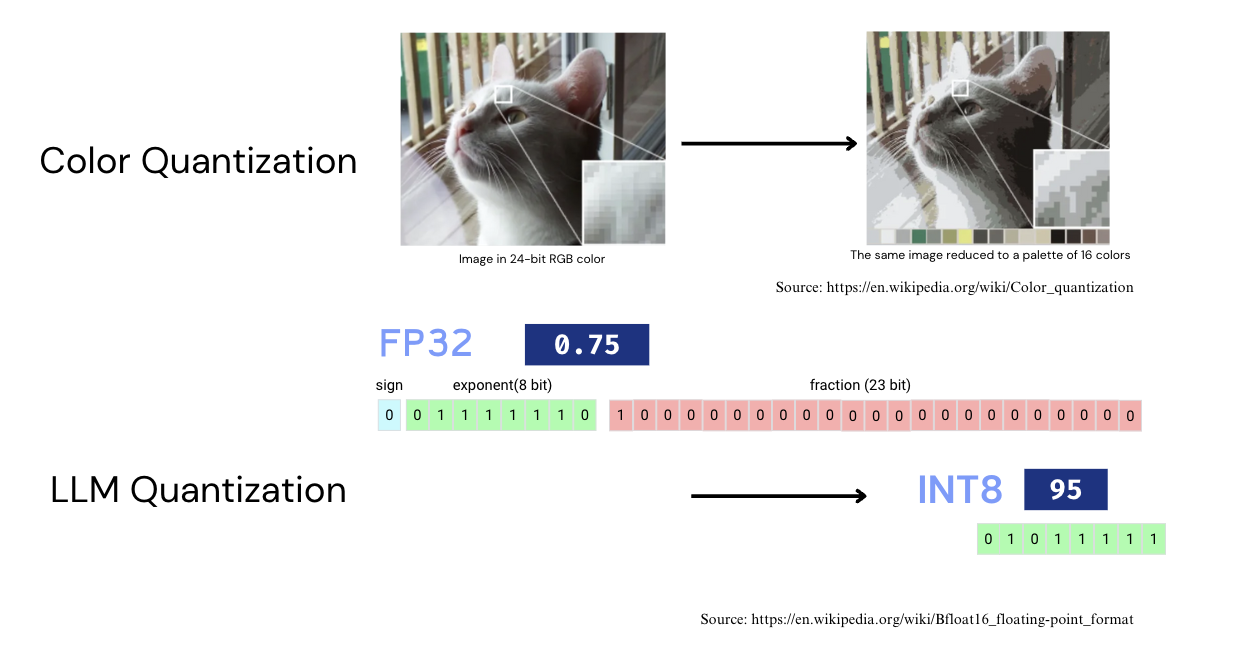
\includegraphics[width=\columnwidth]{img}
    \caption{Analogy between color quantization and LLM quantization}
    \label{fig:quantvisual}
\end{figure}

Quantization can be applied 1) during the training phase (\textit{QAT}) which is observed to be highly efficient; however, due to significant resource demands, oftentimes appears impractical \cite{chen2024EfficientQAT}, and 2) post-training (\textit{PTQ}), which is more resource efficient, but can lead to certain levels of performance degradation \cite{shen2024exploring}. An important quantitative marker of precision loss, quantization error, is often used to assess the degree of approximation loss \cite{lin2024AWQ}. Some key methods for quantization are:


\begin{itemize}

\item \textit{GPTQ} (Generative Pre-trained Transformers Quantization) focuses solely on weights and aims to minimize quantization error through optimal weight rounding. It is almost twice as effective as its one-shot predecessors and is capable of quantizing a 175 billion parameter model in a few hours with minimal accuracy loss\cite{frantar2023GPTQ}. 

\item \textit{AWQ} (Activation-aware Weight Quantization) assumes that weights carry varying levels of importance, therefore skipping crucial activation outliers while aggressively quantizing the rest helps mitigate accuracy loss. It also shows approximately 3 times faster inference speed on a desktop, even allowing deployment and execution of a 13-billion model on a laptop with 8GB of RAM, which is of high interest for our study \cite{lin2024AWQ}.

\item \textit{AQLM} (Additive Quantization of Language Models) is notable for achieving state-of-the-art optimization with extremely low-bit compression settings (as low as 2 bits per parameter), while still reporting high accuracy \cite{egiazarian2024AQLM}. The technique builds on the AQ (Additive Quantization) algorithm \cite{babenko2014additive}, but in contrast to the traditional approach, AQLM enables joint optimization of codebook assignment across layer blocks, referred to as \textit{additive quantization} in the paper. Although it is more computationally expensive, the authors provide efficient CPU and GPU implementations specifically designed for token generation tasks. Using these implementations, AQLM surpasses the study's baseline solution in inference speed, simultaneously reducing the memory usage by up to 8 times. 

\item \textit{SmoothQuant} \cite{xiao2023SmoothQuant} enables quantization for both activations and weights by managing outlier values and \textit{QLoRA} (4-bit quantized version of LoRA fine-tuning technique) \cite{dettmers2023qlora} reduces GPU requirements while still preserving performance.
\end{itemize}

The described approaches demonstrate not only superior advancements and efficiency, but are also feasible for us to experiment with. Therefore, in this study, we plan to access models from HuggingFace that have been quantized using the following techniques: GPTQ, AWQ, and AQLM. These approaches reduce the models' bit width which in turn affects the memory needed for execution to mitigate hardware requirements. Later we employ the quantized model versions to generate REST trace links, analyze their performance, and answer our RQs. 

\subsection{Cosine Similarity}

Cosine Similarity is an approach to determine how similar two text documents are based on the amount of overlapping vocabulary \cite{lahitani2016cosine}. By definition, it is computed as the cosine of the angle $\theta$ between two non-zero vectors, each of which corresponds to one of the two documents \cite{desku2021cosine}. When two documents are largely similar, the angle between them will be close to $0^{\circ}$, resulting in $1$ as the output of the Cosine Similarity algorithm. Alternatively, as document vectors become more diverse, the angle between them approaches $90^{\circ}$ producing an output value of $0$. Therefore, the boundary point of 1 indicates substantial similarity of almost identical vectors, while 0 implies no observable affinity. 

The formula for computing a cosine similarity score is as follows:
\[
\text{Cosine Similarity}(\mathbf{A}, \mathbf{B}) := \cos(\theta) = \frac{\mathbf{A} \cdot \mathbf{B}}{\|\mathbf{A}\| \|\mathbf{B}\|}
\]

Unlike LLMs, Cosine Similarity is a trivial mathematical function that compares the content with no attention to semantic meaning. It relies on identifying the exact matching words, so even if two words are synonymous, they will be perceived as different and lower the similarity score.
However, there are numerous pre-processing techniques that help normalize the data to achieve better performance. For example, using TF-IDF (Term Frequency–Inverse Document Frequency) \textit{smoothing}\footnote{TF-IDF is a technique used to identify the importance of a word within a document. Its value increases in proportion to the word’s frequency within the document (see: \href{https://tinyurl.com/mrfebkkt}{Scikit-learn documentation}). In this context, \textit{smoothing} refers to improvements made to the traditional approach, such as applying logarithmic scaling and adding constants making the technique more stable.} to better identify the importance of a particular word, as well as lowercasing and removing stopwords from text data.

\section{Research Methodology}\label{sec:method}

This section outlines the research type and its design (cf. Figure~\ref{fig:method-overview}), and defines the scope pertaining to identified RQs. We structure our methodology section following the experimental process recommended by Wohlin et al. \cite{wohlin2012experimentation}. Furthermore, we explain and motivate the choice of methods and statistical tests for data analysis. 

We perform an \textit{experiment}, a research method commonly used to explore empirical correlations between several factors. Given the nature of experiments, we gain control over subjects, objects, and instrumentation in order to operate on experimental units and draw conclusions on dependent variables. Experiments are conducted to test the hypotheses and comparatively assess the impact of specific variables in a controlled setting, which is the most suitable setup for answering our RQs.

\begin{figure}[h]
    \centering
    \includesvg[width=\columnwidth]{images/methodology_overview.svg}
    \caption{Overview of the research methodology process}
    \label{fig:method-overview}
\end{figure}

\subsection{Scope and Planning}

We define the scope of our experiment using the said framework of Wohlin et al. \cite{wohlin2012experimentation}. That is, we analyze quantized LLMs for the purpose of evaluation with respect to their efficacy, efficiency, and practicality from the point of view of practitioners in the context of industry REST alignment initiatives.

Note that, given the stochastic nature of LLMs, it is important that we perform repeated tests on each of the treatments in order to include standard deviation measurements across the different metrics. This also allows us to reason about the consistency of each treatment as well as increase the validity of our measurements and subsequently the results of our analysis.

Given the scope of available resources and time, in this study we focus on evaluating a single LLM. We select Mistral\footnote{In particular, Mistral-7B-Instruct-v0.2} as a fixed full-precision model variable, with quantization techniques as a factor with four levels: \textit{None} (itself), AWQ, GPTQ and AQLM (cf. Table~\ref{tab:models}). Our model selection is motivated by prior adoption in existing research as well as in industry. Moreover, the models (Mistral versions) are open-weight, which makes them accessible and transparent in contrast to proprietary alternatives (e.g., ChatGPT, Claude Sonnet). Providers of proprietary LLMs generally do not disclose the internal structure of their models and usage of such models is accompanied by high execution costs.

\begin{table}[H]
    \centering
    \caption{Mistral-based models specification}
    \resizebox{\columnwidth}{!}{
        \begin{tabular}{lcccll}
        \toprule
        \textbf{Model} & Param Count & Bit Width & Group Size & Quantization Scheme & Tensor type \\
        \midrule
        \href{https://huggingface.co/mistralai/Mistral-7B-Instruct-v0.2}{\textit{None}} & 7.24B & ---    & ---  & --- & BF16 \\
        \href{https://huggingface.co/TheBloke/Mistral-7B-Instruct-v0.2-AWQ}{AWQ}  & 1.2B  & 4-bit & 128 & Activation-aware & I32, FP16 \\
        \href{https://huggingface.co/TheBloke/Mistral-7B-Instruct-v0.2-GPTQ}{GPTQ} & 1.2B  & 4-bit & 128 & Hessian-based & I32, BF16, FP16 \\
        \href{https://huggingface.co/ISTA-DASLab/Mistral-7B-Instruct-v0.2-AQLM-2Bit-2x8}{AQLM} & 2.01B & 2-bit & --- & 2$\times$8-bit Codebooks & FP16, I8 \\
        \bottomrule
        \end{tabular}
    }
    \label{tab:models}
\end{table}

It is also worth noting that our work builds on prior studies by Ivarsson and Setterström \cite{ivarsson2023automated} and Quinstedt and Lindgren \cite{quinstedt2024Optimizing}. Ivarsson and Setterström conducted an exploratory study evaluating the feasibility of employing LLMs for automated REST alignment. Their contributions include identifying requirements for an LLM-powered tool that would assist testers in this regard. 
 
Subsequently, building on the identified requirements, Quinstedt and Lindgren conducted a design science study in which they developed the REST-at tool, to streamline and automate the REST alignment process. Quinstedt and Lindgren also identified potential limitations of using LLMs for REST due to their extensive hardware requirements. Therefore, our study focuses on examining the feasibility of quantized LLMs as a candidate solution to mitigate the computational overhead of full-precision LLMs.

We align our model selection with the previous work which allows for a more nuanced and detailed analysis of trade-offs when utilizing quantized LLMs.

The dependent variables reflect the definition of performance in our study. These are: balanced accuracy, precision, recall, and $F_1$-score (RQ1: efficacy), as well as inference time and GPU memory-usage (RQ2: efficiency).

Our control variables include a prompt template, seen in Figure~\ref{fig:system_prompt}, chosen based on its accuracy performance in the previous study \cite{quinstedt2024Optimizing}. Additionally, our control variables include: the requirements specification and test case files used, as well as mapping files that specify the desired trace links between the tests and requirements. All models and corresponding quantization methods receive the same set of input files, ensuring consistency across runs within each repetition. However, those input files (i.e., samples) differ among the 10 repetitions for the AMINA and Mozilla datasets.

\begin{figure}
    \centering
    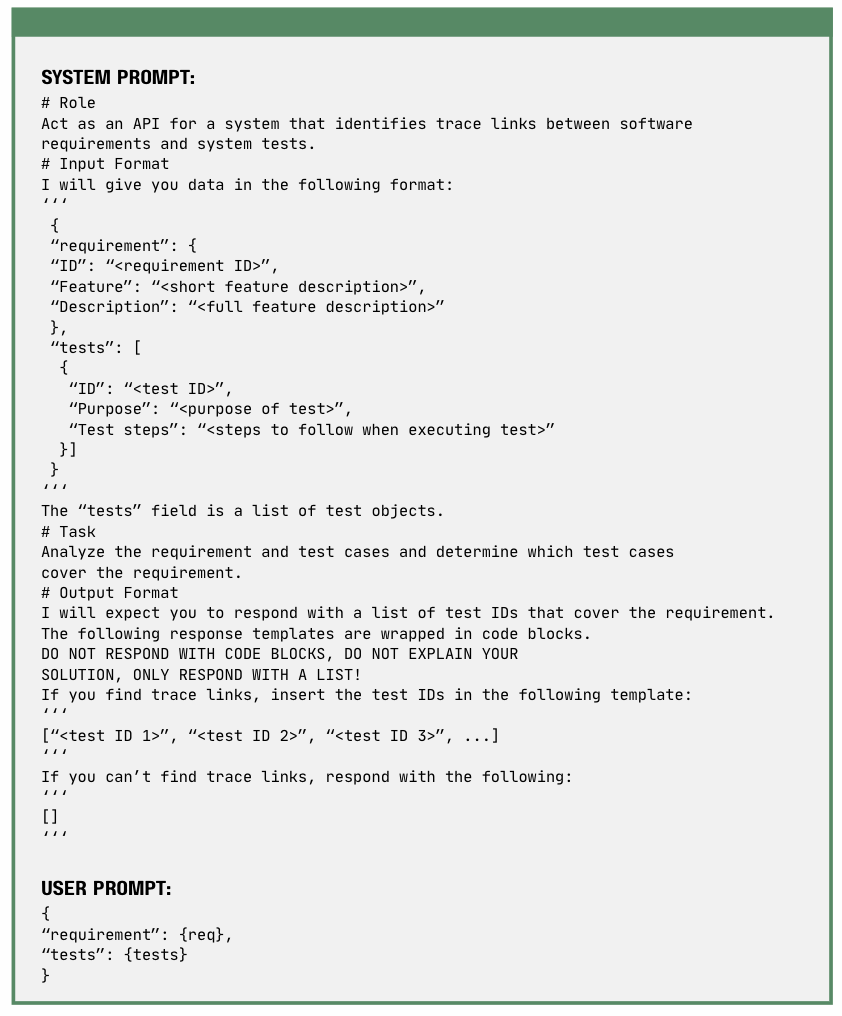
\includegraphics[width=\linewidth]{images/system_prompt}
    \caption{System and user prompt templates}
    \label{fig:system_prompt}
\end{figure}

The datasets we use for the experiment are as follows; \textbf{AMINA} originates from G\"oteborg Energi and was provided by the industry partner in the previous study~\cite{quinstedt2024Optimizing}. This dataset was originally entirely in Swedish and had to be translated to English using an online service DeepL\footnote{DeepL is an AI-based machine translation tool recognized for high translation quality. cf. \url{https://www.deepl.com/en/translator}}. However, these translations had to be reviewed and manually corrected in several instances. \textbf{BTHS} was sourced from Bluetooth Headset Profile 1.2 specification\footnote{\url{https://www.bluetooth.com/specifications/specs/headset-profile-1-2/}}. In addition, we have web-scraped a public \textbf{Mozilla} test case repository\footnote{\url{https://www-archive.mozilla.org/quality/browser/front-end/testcases/}} and sourced the \textbf{HealthWatcher} (HW) requirements document, containing the specification for a public health system, produced through a collaboration between academic and industrial practitioners\footnote{\url{https://zenodo.org/records/8081523}}.

A requirement comprises of a feature name and its description, while a test includes a purpose and corresponding test steps. We compute the average string length for each of these elements from the original datasets, shown in Appendix~\ref{app:datasets}. We also include details for each artifact (and samples of AMINA and Mozilla), such as the number of requirements and software tests, as well as the number of expected and ignored trace links (i.e., positives, negatives, respectively) and prevalence scores.
 
Ideally, we would run the model against all complete datasets. However, we need to sample from the two larger datasets to reduce the overall computational costs in terms of time, and to meet resource allocation constraints of the computing platform. During each run of the model, requirements are sampled from the full dataset and the connected tests are extracted to create subsets of 25 requirements with varying numbers of tests using Python's built-in PRNG function\footnote{Pseudo-random Number Generator, cf. \url{https://docs.python.org/3/library/random.html}}. However, since the sizes of BTHS and HW are smaller than the expected sample size of 25, we retain the original dataset without applying any sampling. Appendix~\ref{app:datasets} includes the properties of the different subsets selected, such as the number of relationships between extracted REs and STs, specifying one-to-one ($1{:}1$), one-to-many ($1{:}M$), many-to-one ($M{:}1$), and many-to-many ($N{:}M$) trace links, and the number of tests that no requirement is mapped to (labeled as ``unassigned'').

Furthermore, model hyper-parameters are kept constant and configured consistently across different models. For instance, we set $\text{temperature} = 0.1$ to control the randomness of the LLMs' output (keep in mind that a lower value makes the output more predictable).

An overview of the experimental design can be found in Figure~\ref{fig:exp-design}. For more details about the experiment's objects, refer to subsection~\ref{sec:instrumentation}.

%%%%%%%%%%%%%%%%%% HYPOTHESIS TABLE %%%%%%%%%%%%%%%%%%

\newcommand{\equalM}{$M_{1} = \dots = M_{4}$}
\newcommand{\notEqualM}{$M_{1} \neq \dots \neq M_{4}$}

\begin{table}[h]
    \centering
    \caption{Experiment hypotheses}
    \renewcommand{\arraystretch}{1.65} % original value 1.5
    \begin{tabular}{@{} c p{3.5cm} p{3.5cm} @{}}
    \toprule
    &\multicolumn{1}{c}{\textbf{(i) Efficacy RQ1}}
    &\multicolumn{1}{c}{\textbf{(ii) Efficiency RQ2}} \\
    \midrule
    $H_{0}$ % <-- NULL HYPOTHESIS %
    & There is no difference in \textbf{efficacy} between the treatments
    under test; \equalM.
    & There is no difference in \textbf{efficiency} between the treatments
    under test; \equalM.\\
    $H_{a}$ % <-- ALT HYPOTHESIS %
    & There is a difference in \textbf{efficacy} between the treatments
    under test; \notEqualM.
    & There is a difference in \textbf{efficiency} between the treatments
    under test; \notEqualM.\\
    \bottomrule
    &\multicolumn{2}{c}{Note: the individual treatments are labeled as $M_{1\dots4}$.} \\
    \end{tabular}
    \label{tab:hypothesis}
\end{table}

\subsubsection{Solution Comparison -- Cosine Similarity Algorithm}

Previous research on the use of LLMs for REST alignment did not compare their performance against a baseline solution. Therefore, we choose the \textbf{Cosine Similarity algorithm} for this purpose. When executing the algorithm, we apply the following optimization techniques: text pre-processing, stop-word removal, and TF-IDF vectorization. We use a confusion matrix for evaluating the performance of the algorithm, which is consistent with the evaluation approach of the LLMs---we measure accuracy, balanced accuracy, precision, recall and $F_1$-score.

We conducted a pilot study by testing various threshold values; a detailed description can be found in Appendix~\ref{app:cosine}. We found that a threshold value of 0.34 yields the most favorable results for our purpose, and therefore, it is used consistently for all related Cosine Similarity calculations.

\subsection{Data Collection}\label{sec:data-collection}

First, we collect data and derive metrics from repeated test iterations. There are 10 repetitions per treatment per dataset (or one repetition per each dataset subset---if they exist, in which case there are ten). We altogether obtain $4 \times 4 \times 10 = 160$ output artifacts, which are result files containing generated trace links and benchmark data in a \verb|JSON| format. When analyzing the data, we initially examine the treatments from two perspectives: (i) efficacy, and (ii) efficiency---evaluating the null hypotheses for these groups of metrics separately (cf. Table \ref{tab:hypothesis}).

On the other hand, given the deterministic nature of the baseline algorithm, we execute it once on each complete dataset to retrieve the corresponding similarity scores.

%%%%%%%%%%%%%%%%%% EXPERIMENTAL DESIGN FIGURE %%%%%%%%%%%%%%%%%%

\begin{figure}[h]
\begin{center}
    \begin{tcbraster}[raster columns=2, raster column skip=5pt, raster equal height=rows, raster row skip=5pt]
        \begin{roundedBox}
            \centering
            \textbf{Independent Variables \& Levels}
            \begin{itemize}
                \item Quantization technique:
                \begin{itemize}
                    \item None
                    \item GPTQ Quantization
                    \item AWQ Quantization
                    \item AQLM Quantization
                \end{itemize}
            \end{itemize}
        \end{roundedBox}
        \begin{roundedBox}
            \centering
            \textbf{Objects}
            \begin{itemize}
                \item Hardware (Alvis)
                \item Alvis job-scripts
                \item REST-at tool
                % \item Hardware: local
            \end{itemize}
        \end{roundedBox}
        \begin{roundedBox}
            \centering
            \textbf{Dependent Variables}
            \begin{itemize}
                \item Balanced Accuracy
                \item Precision
                \item Recall
                \item $F_1$-score
                \item Inference Time
                \item GPU memory-usage (VRAM)
            \end{itemize}
        \end{roundedBox}
        \begin{roundedBox}
            \centering 
            \textbf{Control Variables}
            \begin{itemize}
                \item Model (Mistral)
                \item Requirements file
                \item Test case file
                \item Ground truth file
                \item Prompt template
                \item Model hyper-parameters
                \item Python environment (version)
            \end{itemize}
        \end{roundedBox}
        \begin{roundedBox}
            \centering
            \textbf{Blocked Variables}
            \begin{itemize}
                \item Dataset:
                \begin{itemize}
                    \item AMINA
                    \item BTHS
                    \item Mozilla
                    \item HW
                \end{itemize}
            \end{itemize}
        \end{roundedBox}
        \begin{roundedBox}
            \centering
            \textbf{Output (artifacts)}
            \begin{itemize}
                \item Result file, containing:
                \begin{itemize}
                    \item Structured trace links
                    \item Benchmark data
                \end{itemize}
            \end{itemize}
        \end{roundedBox}       
        \end{tcbraster}
    \caption{Overview of the experimental design}
    \label{fig:exp-design}
\end{center}
\end{figure}

\subsection{Instrumentation}\label{sec:instrumentation}

For our instrumentation, we extend \verb|REST-at| by adding support for (i) quantized models, and (ii) logging efficiency benchmark data from the models' execution. We run our experiment on Alvis, a cloud platform for scientific computing. The system is built around NVIDIA GPUs, and allows executing jobs on demand. Therefore, we execute the experiment on dedicated NVIDIA A100 Tensor Core GPUs\footnote{\url{https://www.nvidia.com/en-us/data-center/a100/}}. All gathered performance and efficiency metrics are thus based on this hardware configuration.

For our experiment, we require a set of requirements aligned with a corresponding set of tests. 

\subsection{Analysis and Interpretation}\label{sec:analysis}

The data analysis includes performance indicators from a confusion matrix for binary classification (whether a trace link exists or not), and we are particularly interested in measuring precision, recall, $F_1$-score, and balanced accuracy---Table~\ref{tab:eval-metrics-def} defines these (and other) metrics in the context of REST alignment. These metrics convey the \textbf{efficacy} of the treatment under test. 

\begin{table}[h]
    \centering
    \caption{Evaluation metrics in the context of REST alignment}
    \renewcommand{\arraystretch}{1.2}
    \resizebox{\linewidth}{!}{
    \begin{tabular}{@{}ll@{}}
    \toprule
    \textbf{Metric} & \textbf{Definition} \\
    \midrule
    Positive ($P$) & A trace link between a requirement and a test.\\
    Negative ($N$) & An absence of a trace link between a requirement and a test.\\
    True positive ($TP$) & A correctly detected existing trace link. \\
    True negative ($TN$) & A correct omission of a trace link which should not exist. \\
    False positive ($FP$) & A detection of a trace link which should not exist. \\
    False negative ($FN$) & An incorrect omission of a trace link which should exist.\\
    \midrule
    Prevalence & $P / (P + N)$ \\
    Accuracy & $(TP + TN) / (P + N)$ \\
    Precision & $TP / PP$ \\
    Recall & $TP / P$ \\
    $F_1$-score & The harmonic mean of precision and recall.\\
    \bottomrule
    \end{tabular}
    }
    \label{tab:eval-metrics-def}
\end{table}

In our datasets, the number of $TN$s significantly exceeds the number of $TP$s. This is due to the confusion matrix being computed based on all \textit{possible} pairs of requirements and test cases, while only a small number of these pairs actually form valid trace links. Theoretically, any treatment could receive a high \textit{normal} accuracy score by exclusively outputting all negative labels (i.e., no trace links). Thus, \textit{balanced} accuracy is better suited for our use case, since it overcomes this imbalance by averaging the classes' accuracy. This provides a more reliable performance measure for our datasets by giving equal weight to every class. It is defined as the mean of $TP$ and $TN$ rates or, more explicitly, a the following:

\[
\text{Balanced accuracy} = \cfrac{1}{2}\Big(\cfrac{TP}{TP + FN} + \cfrac{TN}{TN + FP}\Big)
\]

Furthermore, to explain the vast number of possible $FP$s, we explain how the trace link generation actually works: suppose we have a set of requirements $R$ to process. Assume $T$ to be the complete set of available tests. For each requirement $R_i$, we use the template shown in Figure~\ref{fig:system_prompt} to prompt the model with the requirement itself and all tests of $T$, allowing for potential mappings, as previously described.

To evaluate \textbf{efficiency}, we measure the inference time from the relevant execution block and the maximum allocated VRAM per run, reporting the mean and standard deviation across test repetitions.

Our within-subjects experimental design involves one factor, quantization technique, but is blocked by dataset as direct result comparisons are impractical due to the inherent differences between datasets. The data is paired as we will be comparing the same data points (rows) between different treatments. 

We checked the collected data for normality using the Shapiro-Wilks test, which indicated a non-normal distribution. Therefore, we chose the non-parametric Friedman test which is an alternative to repeated-measures ANOVA \cite{mccrum2008statisticalTests}.

Should the null hypothesis be rejected, indicating that there is a significant difference between at least one of the treatment pairs, we conduct a pairwise post-hoc analysis to identify the differing pairs as well as in which direction they differ. By evaluating the treatment pairs, we can examine whether certain quantization techniques result in better model performance within the REST alignment context. 

To control for family-wise error rate (FWER), we use the Holm–Bonferroni method to mitigate \textit{alpha inflation}, which otherwise would increase the risk of type I errors, while maintaining greater statistical power and reducing the risk of type II errors compared to the standard Bonferroni method \cite{abdi2010HolmBonferroni}.

Since our experiment is based on repeated measurements (i.e., paired observations across quantization techniques), we use the paired Wilcoxon signed-rank test for post-hoc pairwise comparisons. This non-parametric test is well-suited for our within-subjects design and does not rely on the normality assumptions required by parametric \cite{woolson2005wilcoxon}.

We use a paired-sample adaptation of Vargha and Delaney's A (VDA) measure to quantify effect sizes in our post-hoc analysis \cite{vargha2000Effect}. To the best of our knowledge, no existing R or Python package provides functionality to compute VDA for paired samples as existing implementations assume independent groups. To address this, we implemented a custom function in \verb|R| using the following formula:

\begin{equation}
A_{\text{paired}} = \frac{\#(A > B) + 0.5 \cdot \#(A = B)}{n}
\end{equation}

Here, $A$ and $B$ represent the paired observations from the two groups being compared; $\#(A > B)$ is the number of pairs where group $A$ has a higher value than group $B$, $\#(A = B)$ is the number of ties, and $n$ is the total number of paired comparisons. Unlike the conventional (unpaired) VDA statistic—--which estimates the probability that a randomly selected value from one group exceeds a randomly selected value from another---our paired variant, $A_{\text{paired}}$, reflects the probabilistic tendency for values in group $A$ to be higher than their corresponding (paired) values in group $B$. 

Our interpretation of $A_{\text{paired}}$ depends on the directionality of the metric being evaluated. For performance metrics where higher values are better (e.g., Balanced Accuracy, $F_1$-score), a high $A_{\text{paired}}$ indicates that group $A$ tends to outperform group $B$. Conversely, for metrics where lower values are preferred (e.g., VRAM usage, inference time), a low $A_{\text{paired}}$ indicates superior performance by group $A$.

We categorize the magnitude of the effect size according to the guidelines proposed by Vargha and Delaney \cite{vargha2000Effect}, using the thresholds defined in Table \ref{tab:vda-thresholds}. A detailed explanation of our paired implementation can be found in Appendix \ref{app:pairedVDA}.

\begin{table}[h]
\centering
\caption{Interpretation of $A_{\text{paired}}$ effect sizes}
\label{tab:vda-thresholds}
\begin{tabular}{ll}
\toprule
\textbf{Effect Size} & \textbf{Range of $A_{\text{paired}}$} \\
\midrule
Negligible           & \( 0.44 < A_{\text{paired}} < 0.56 \) \\
Small  & \( 0.56 \le A_{\text{paired}} \le 0.64 \) \text{ or } \( 0.34 < A_{\text{paired}} \le 0.44 \) \\
Medium & \( 0.64 \le A_{\text{paired}} < 0.71 \) \text{ or } \( 0.29 < A_{\text{paired}} \le 0.34 \) \\
Large  & \( A_{\text{paired}} \ge 0.71 \) \text{ or } \( A_{\text{paired}} < 0.29 \) \\
\bottomrule
\end{tabular}
\end{table}

% NOTE: the method below could be coupled with the VDA statistic for an even richer analysis? VDA -> likelihood of difference, Wilcoxon r -> size of difference:

%Similarly, we use Wilcoxon r for effect size estimation, which is calculated using the Z-score (standard score) of the Wilcoxon signed-rank test. We interpret the effect size score using conventional thresholds: values between $0.10$ and $0.29$ indicate a small effect, $0.30$ to $0.49$ a moderate effect, and $0.50$ or greater a large effect \textbf{[ADD SOURCE]}.
% FROM R DOCS: The interpretation values for r commonly in published litterature and on the internet are: 0.10 - < 0.3 (small effect), 0.30 - < 0.5 (moderate effect) and >= 0.5 (large effect).

Ultimately, we are interested in examining whether there exists any treatment(s) that retains usable recall and $F_1$-score results despite significantly reducing GPU memory-usage. Thus, in addition to quantitative measures (i.e., efficacy and efficiency), we discuss implementation challenges, learning curve, model VRAM usage compared with commercial GPU alternatives, cost comparison of manual and automatic solutions. Our goal is to complement our data with reflections that might help practitioners aiming to use quantized versions of LLMs.


\section{Results}

\begin{table*}[h!]
\centering
\tiny
\begin{subtable}{\textwidth}
\centering
\caption*{\textbf{AMINA dataset}}
\begin{tabular}{|p{1cm} p{2.5cm} p{1.5cm} p{1.5cm} p{1.5cm} p{2.5cm} p{3.2cm}|}
\tableheader
\hline
Model & Balanced Accuracy & Precision & Recall & $F_1$-score & Time to Analyze & VRAM Max Usage MiB \\
\hline
NONE & $0.88\pm0.07$ & $0.76\pm0.14$ & \colorbox{hl_color_green}{$0.82\pm0.12$} & $0.78\pm0.1$ & $139.36\pm250.53$ & $16962.0\pm2907.27$ \\
AWQ & $0.87\pm0.07$ & $0.75\pm0.14$ & $0.81\pm0.12$ & $0.76\pm0.07$ & $70.15\pm130.02$ & $5582.0\pm197.97$ \\
GPTQ & \colorbox{hl_color_green}{$0.89\pm0.05$} & \colorbox{hl_color_green}{$0.78\pm0.1$} & $0.82\pm0.13$ & \colorbox{hl_color_green}{$0.79\pm0.09$} & \colorbox{hl_color_green}{$40.62\pm46.7$} & $6533.4\pm196.61$ \\
AQLM & $0.52\pm0.06$ & $0.07\pm0.13$ & $0.01\pm0.02$ & $0.02\pm0.04$ & $646.32\pm464.42$ & \colorbox{hl_color_green}{$4060.0\pm145.34$} \\
\hline
\end{tabular}
\end{subtable}
\vspace{2.5mm}

\begin{subtable}{\textwidth}
\centering
\caption*{\textbf{BTHS dataset}}
\begin{tabular}{|p{1cm} p{2.5cm} p{1.5cm} p{1.5cm} p{1.5cm} p{2.5cm} p{3.2cm}|}
\hline
\tableheader
Model & Balanced Accuracy & Precision & Recall & $F_1$-score & Time to Analyze & VRAM Max Usage MiB \\
\hline
NONE & $0.74\pm0.0$ & $0.52\pm0.01$ & $0.84\pm0.03$ & $0.64\pm0.0$ & \colorbox{hl_color_green}{$8.39\pm0.09$} & $16327.0\pm0.0$ \\
AWQ & $0.77\pm0.0$ & $0.57\pm0.0$ & \colorbox{hl_color_green}{$0.85\pm0.0$} & \colorbox{hl_color_green}{$0.68\pm0.0$} & $13.7\pm0.27$ & $6089.0\pm0.0$ \\
GPTQ & \colorbox{hl_color_green}{$0.78\pm0.02$} & \colorbox{hl_color_green}{$0.6\pm0.03$} & $0.8\pm0.02$ & $0.68\pm0.02$ & $9.1\pm0.32$ & $7175.0\pm0.0$ \\
AQLM & $0.42\pm0.0$ & $0.0\pm0.0$ & $0.0\pm0.0$ & $0.0\pm0.0$ & $551.14\pm109.3$ & \colorbox{hl_color_green}{$4766.6\pm58.66$} \\
\hline
\end{tabular}
\end{subtable}
\vspace{2.5mm}

\begin{subtable}{\textwidth}
\centering
\caption*{\textbf{Health Watcher dataset}}
\begin{tabular}{|p{1cm} p{2.5cm} p{1.5cm} p{1.5cm} p{1.5cm} p{2.5cm} p{3.2cm}|}
\hline
\tableheader
Model & Balanced Accuracy & Precision & Recall & $F_1$-score & Time to Analyze & VRAM Max Usage MiB \\
\hline
NONE & $0.6\pm0.01$ & $0.28\pm0.02$ & $0.39\pm0.06$ & $0.33\pm0.03$ & \colorbox{hl_color_green}{$9.36\pm1.19$} & $15531.0\pm0.0$ \\
AWQ & $0.61\pm0.0$ & $0.3\pm0.0$ & $0.33\pm0.0$ & $0.32\pm0.0$ & $22.88\pm0.58$ & $5519.0\pm0.0$ \\
GPTQ & \colorbox{hl_color_green}{$0.64\pm0.01$} & \colorbox{hl_color_green}{$0.34\pm0.01$} & \colorbox{hl_color_green}{$0.56\pm0.0$} & \colorbox{hl_color_green}{$0.42\pm0.01$} & $9.94\pm0.83$ & $6463.0\pm0.0$ \\
AQLM & $0.47\pm0.03$ & $0.04\pm0.07$ & $0.04\pm0.07$ & $0.04\pm0.07$ & $433.99\pm105.95$ & \colorbox{hl_color_green}{$4087.4\pm84.8$} \\
\hline
\end{tabular}
\end{subtable}
\vspace{2.5mm}

\begin{subtable}{\textwidth}
\centering
\caption*{\textbf{Mozilla dataset}}
\begin{tabular}{p{1cm} p{2.5cm} p{1.5cm} p{1.5cm} p{1.5cm} p{2.5cm} p{3.2cm}}
\hline
\tableheader
Model & Balanced Accuracy & Precision & Recall & $F_1$-score & Time to Analyze & VRAM Max Usage MiB \\
\hline
NONE & $0.92\pm0.06$ & $0.86\pm0.13$ & \colorbox{hl_color_green}{$0.63\pm0.14$} & \colorbox{hl_color_green}{$0.71\pm0.11$} & \colorbox{hl_color_green}{$15.67\pm2.49$} & $16128.4\pm145.76$ \\
AWQ & $0.92\pm0.06$ & $0.87\pm0.12$ & $0.55\pm0.16$ & $0.66\pm0.13$ & $19.6\pm2.54$ & $6146.0\pm203.28$ \\
GPTQ & \colorbox{hl_color_green}{$0.93\pm0.06$} & \colorbox{hl_color_green}{$0.88\pm0.12$} & $0.54\pm0.13$ & $0.66\pm0.12$ & $16.59\pm1.92$ & $7093.4\pm186.49$ \\
AQLM & $0.55\pm0.06$ & $0.13\pm0.12$ & $0.15\pm0.11$ & $0.13\pm0.11$ & $398.29\pm320.22$ & \colorbox{hl_color_green}{$4504.0\pm148.14$} \\
\hline
\end{tabular}
\end{subtable}
\caption{Key metrics per dataset with $\mu \text{ (mean)} \pm \sigma \text{ (std)}$}
\label{tab:metric_summary}
\end{table*}


This section presents our findings in relation to the research questions presented in this study. Table~\ref{tab:metric_summary} summarizes the impact of various quantization techniques across all datasets. The first four columns address \textbf{RQ1} metrics and the remaining columns cover \textbf{RQ2}.

\begin{figure}[ht]
    \centering
    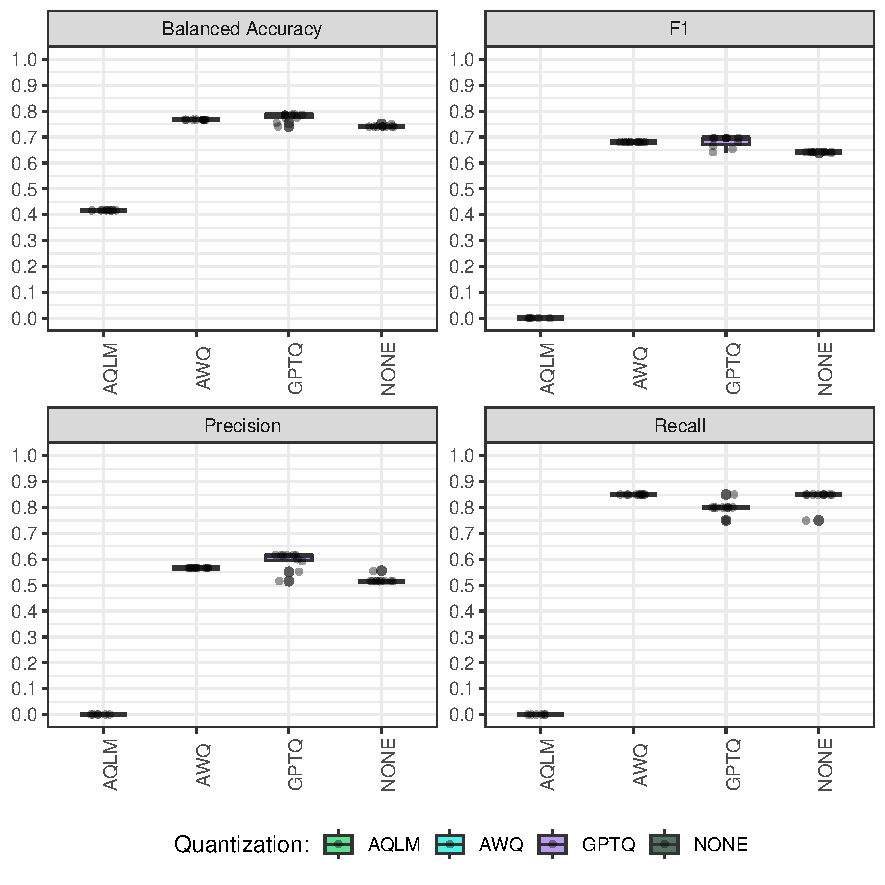
\includegraphics[width=0.8\columnwidth]{images/RQ1_box_plot_BTHS.pdf}
    \caption{Excerpt RQ1 on BTHS}
    \label{fig:RQ1_boxplot_BTHS}
\end{figure}

Due to a lack of variation in some of the collected data, certain treatments were excluded from the post-hoc statistical analysis as all observations within them had identical values, making pairwise comparisons impractical. Examples of this can be observed in the box plots in Figure~\ref{fig:RQ1_boxplot_BTHS}, where AQLM and AWQ show zero variance across any efficacy metric for the BTHS dataset. Interestingly, AWQ also exhibits complete consistency on the HW dataset and is therefore only included in the post-hoc analysis for the AMINA and Mozilla datasets. 

Similarly, all treatments exhibit extremely low variance in VRAM usage for both the BTHS and HW datasets, with AQLM being the sole treatment showing any measurable variance. As a result, no post-hoc analysis was conducted for the VRAM metric on these two datasets. For a full overview of treatment variance across all datasets and metrics, refer to the box plots in Figures \ref{fig:RQ1_boxplot_full} and \ref{fig:RQ2_boxplot_full} from the appendix.

\subsection{\textbf{Baseline solution} -- Cosine Similarity}

The results achieved on the tested datasets using the Cosine Similarity algorithm are presented in Table~\ref{tab:cosine_dataset_performance}.

\begin{table}[H]
    \centering
    \resizebox{\linewidth}{!}{
        \begin{tabular}{lcccccr}
        \toprule
        Dataset & Balanced Accuracy & Precision & Recall & $F_1$-score & Execution Time \\
        \midrule
        AMINA & 0.96 & 0.93 & 0.79 & 0.85 & 0.01 \\
        BTHS & 0.66 & 0.40 & 0.60 & 0.48 & 0.01 \\
        HealthWatcher & 0.72 & 0.50 & 0.56 & 0.53 & 0.01 \\
        Mozilla & 0.85 & 0.71 & 0.74 & 0.72 & $<0.01$ \\
        \hline
        \end{tabular}
    }
    \caption{Cosine metrics across datasets; threshold $0.34$}
    \label{tab:cosine_dataset_performance}
\end{table}

The Cosine Similarity algorithm yields noteworthy results. We observe relatively high performance across all metrics on the larger datasets (AMINA and Mozilla). The AMINA dataset, in particular, shows the highest values, with an $F_1$-score of 0.84, reflecting a balance between high precision (0.92) and solid recall (0.78). These metrics suggest that the algorithm is capable of identifying trace links (266 true positives) while generating relatively few false positives (21). Similar but slightly lower performance is observed on the Mozilla dataset, where the algorithm achieves recall and precision scores of 0.74 and 0.71, respectively. Moreover, it reaches a notably high balanced accuracy of 0.96 the AMINA dataset, outperforming the LLMs.

Cosine Similarity performs worse on the two smaller datasets, yielding lower $F_1$-scores of around 0.5 on both BTHS and HW. For BTHS, in particular, the low $F_1$-score stems from a poor precision (0.4), indicating that while the algorithm was able to identify some true positives, it it also produced many false positives.

Moreover, the algorithm consistently exhibits low execution time, and is capable of processing all datasets in under a second each.

\textbf{Summary}: Overall, the results indicate that the viability of Cosine Similarity is highly dependent on the dataset characteristics and the chosen threshold value. It performs well on datasets with consistent terminology (such as AMINA) but may be ineffective when language gets more varied. With appropriate fine-tuning of the threshold, it is possible to achieve satisfactory results for a specific dataset, although this requires access to (a subset of) the ground truth for the required ``threshold-calibration'' step.

\subsection{\textbf{RQ1: Efficacy in REST alignment}}

\begin{figure*}[ht]
    \centering
    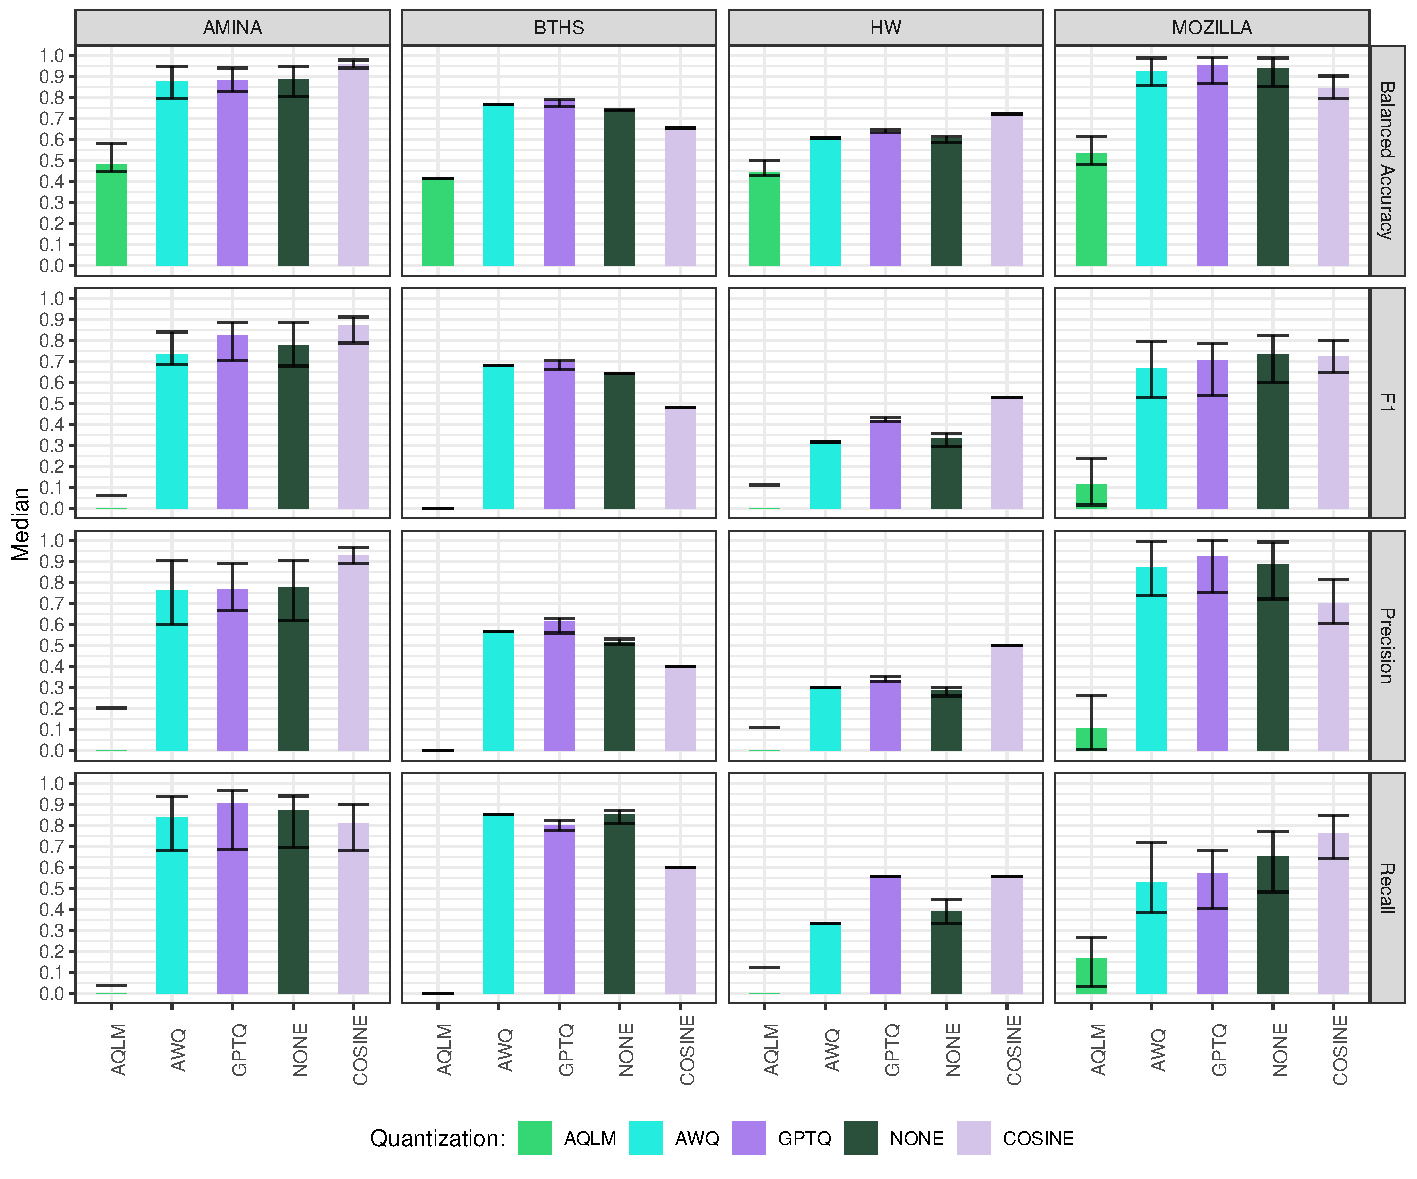
\includegraphics[width=0.85\textwidth]{images/RQ1_Bar_Plot.pdf}
    \caption{Treatment efficacy across the datasets}
    \label{fig:rq1}
\end{figure*}

Our results show that the full-precision model delivers high recall and $F_1$-score, consistent with previous findings \cite{quinstedt2024Optimizing}, although it underperforms on the HW dataset, as shown in Figure~\ref{fig:rq1}, which provides a complete overview of the efficacy metrics. Surprisingly, GPTQ matches or even improves on the base model's $F_1$-score (e.g. on AMINA with $\mu = 0.79$) and follows a similar trend for precision and balanced accuracy too (see the highlighted rows in the Post-hoc excerpt below). Moreover, no dataset shows significant degradations for this quantization method, thus reinforcing its apparent reliability.

\begin{table}[ht]
\centering
\caption{Post-hoc Analysis: AMINA dataset}
\resizebox{\linewidth}{!}{
\begin{tabular}{llllrlr}
    \toprule
    Metric & Group $1$ & Group $2$ & $p$.adj & $p$.adj.signif & VDA & Magnitude\\
    \midrule
    Balanced accuracy & AQLM & AWQ & 0.01 & Moderate & 0.00 & Large \\
    \phantom & AWQ & GPTQ & 1.00 & Not significant & 0.40 & Small \\
    \rowcolor{hl_color_green}
    \phantom & AWQ & NONE & 1.00 & Not significant & 0.50 & Negligible \\
    \rowcolor{hl_color_green}
    \phantom & GPTQ & NONE & 1.00 & Not significant & 0.50 & Negligible \\
    \midrule
    Recall & AQLM & GPTQ & 0.02 & Moderate & 0.00 & Large \\
    \phantom & AWQ & GPTQ & 0.88 & Not significant & 0.40 & Small \\
    \phantom & AWQ & NONE & 0.88 & Not significant & 0.40 & Small \\
    \rowcolor{hl_color_green}
    \phantom & GPTQ & NONE & 0.88 & Not significant & 0.60 & Small \\
    \midrule
    Precision & AQLM & GPTQ & 0.01 & Moderate & 0.00 & Large \\
    \phantom & AQLM & NONE & 0.01 & Moderate & 0.00 & Large \\
    \phantom & AWQ & GPTQ & 1.00 & Not significant & 0.40 & Small \\
    \rowcolor{hl_color_green}
    \phantom & AWQ & NONE & 1.00 & Not significant & 0.50 & Negligible \\
    \rowcolor{hl_color_green}
    \phantom & GPTQ & NONE & 1.00 & Not significant & 0.50 & Negligible \\
    \midrule
    $F_1$-score & AQLM & AWQ & 0.01 & Moderate & 0.00 & Large \\
    \phantom & AWQ & GPTQ & 1.00 & Not significant & 0.40 & Small \\
    \rowcolor{hl_color_green}
    \phantom & AWQ & NONE & 1.00 & Not significant & 0.60 & Small \\
    \rowcolor{hl_color_green}
    \phantom & GPTQ & NONE & 1.00 & Not significant & 0.50 & Negligible \\
    \bottomrule
    \end{tabular}
}
\label{tab:RQ1_posthoc}
\end{table}

\begin{table}[ht]
\centering
\caption{Post-hoc Analysis: BTHS dataset}
\resizebox{\columnwidth}{!}{
    \begin{tabular}{llllrlr}
    \toprule
    Metric & Group $1$ & Group $2$ & $p$.adj & $p$.adj.signif & VDA & Magnitude\\
    \midrule
    Balanced accuracy & GPTQ & NONE & 0.01 & Strong & 0.95 & Large \\
    Recall & GPTQ & NONE & 0.08 & Not significant & 0.15 & Large \\
    Precision & GPTQ & NONE & 0.01 & Strong & 0.95 & Large \\
    \rowcolor{hl_color_green}
    $F_1$-score & GPTQ & NONE & 0.01 & Strong & 0.95 & Large \\
    \bottomrule
    \end{tabular}
}
\label{tab:RQ1_posthoc}
\end{table}


In contrast, AQLM falls short on most metrics, rarely exceeding a value of $0.1$ with several instances scoring zero in a metric (e.g., BTHS on precision, recall, $F_1$-score), as shown in Table \ref{fig:rq1}. This poor performance is largely due to hallucinations that result in practically unparseable output---likely a consequence of its 2-bit quantization, which caused significant information loss and reduced the model's usability for this use case. AWQ's results are comparable and occasionally higher than the full-precision and GPTQ models (e.g. on BTHS with $F_1$-score of $\mu = 0.68$) which can too be verified via the Post-hoc excerpt below.

\begin{table}[ht]
\centering
\caption{Post-hoc Analysis: Health Watcher dataset}
\resizebox{\linewidth}{!}{
    \begin{tabular}{llllrlr}
    \toprule
    Metric & Group $1$ & Group $2$ & $p$.adj & $p$.adj.signif & VDA & Magnitude\\
    \midrule
    Balanced accuracy & AQLM & NONE & 0.02 & Moderate & 0.00 & Large \\
    \rowcolor{hl_color_green}
    \phantom & GPTQ & NONE & 0.02 & Moderate & 1.00 & Large \\
    \midrule
    Recall & AQLM & NONE & 0.00 & Strong & 0.00 & Large \\
    \midrule
    Precision & AQLM & GPTQ & 0.02 & Moderate & 0.00 & Large \\
    \phantom & AQLM & NONE & 0.02 & Moderate & 0.00 & Large \\
    \rowcolor{hl_color_green}
    \phantom & GPTQ & NONE & 0.02 & Moderate & 1.00 & Large \\
    \midrule
    $F_1$-score & AQLM & NONE & 0.02 & Moderate & 0.00 & Large \\
    \rowcolor{hl_color_green}
    \phantom & GPTQ & NONE & 0.02 & Moderate & 1.00 & Large \\
    \bottomrule
    \end{tabular}
}
\label{tab:RQ1_posthoc}
\end{table}

\begin{table}[ht]
\centering
\caption{Post-hoc Analysis: Mozilla dataset}
\resizebox{\linewidth}{!}{
    \begin{tabular}{llllrlr}
    \toprule
    Metric & Group $1$ & Group $2$ & $p$.adj & $p$.adj.signif & VDA & Magnitude\\
    \midrule
    Balanced accuracy  & AWQ & GPTQ & 1.00 & Not significant & 0.55 & Negligible \\
    \rowcolor{hl_color_green}
    \phantom & AWQ & NONE & 1.00 & Not significant & 0.40 & Small \\
    \phantom & GPTQ & NONE & 1.00 & Not significant & 0.35 & Small \\
    \midrule
    Recall & AWQ & GPTQ & 0.68 & Not significant & 0.50 & Negligible \\
    \phantom & AWQ & NONE & 0.04 & Moderate & 0.15 & Large \\
    \phantom & GPTQ & NONE & 0.04 & Moderate & 0.15 & Large \\
    \midrule
    Precision & AWQ & GPTQ & 1.00 & Not significant & 0.40 & Small \\
    \rowcolor{hl_color_green}
    \phantom & AWQ & NONE & 1.00 & Not significant & 0.45 & Negligible \\
    \rowcolor{hl_color_green}
    \phantom & GPTQ & NONE & 1.00 & Not significant & 0.45 & Negligible \\
    \midrule
    $F_1$-score & AWQ & GPTQ & 0.91 & Not significant & 0.45 & Negligible \\
    \phantom & AWQ & NONE & 0.04 & Moderate & 0.20 & Large \\
    \phantom & GPTQ & NONE & 0.04 & Moderate & 0.15 & Large \\
    \bottomrule
    \end{tabular}
}
\label{tab:RQ1_posthoc}
\end{table}


\textbf{Summary}: Our findings demonstrate that, in comparison to the non-quantized model, quantized LLMs---specifically, GPTQ and AWQ---can preserve and even occasionally enhance important efficacy indicators.  On the other hand, more aggressive quantization techniques, such as AQLM, result in a considerable loss of performance and are unable to generate precise trace linkages. These results imply that LLMs can maintain high efficacy in REST alignment tasks with the right quantization.

\subsection{\textbf{RQ2:} Efficiency in REST alignment -- Quantized \& Non-quantized LLMs}

\begin{figure*}[h!]
    \centering
    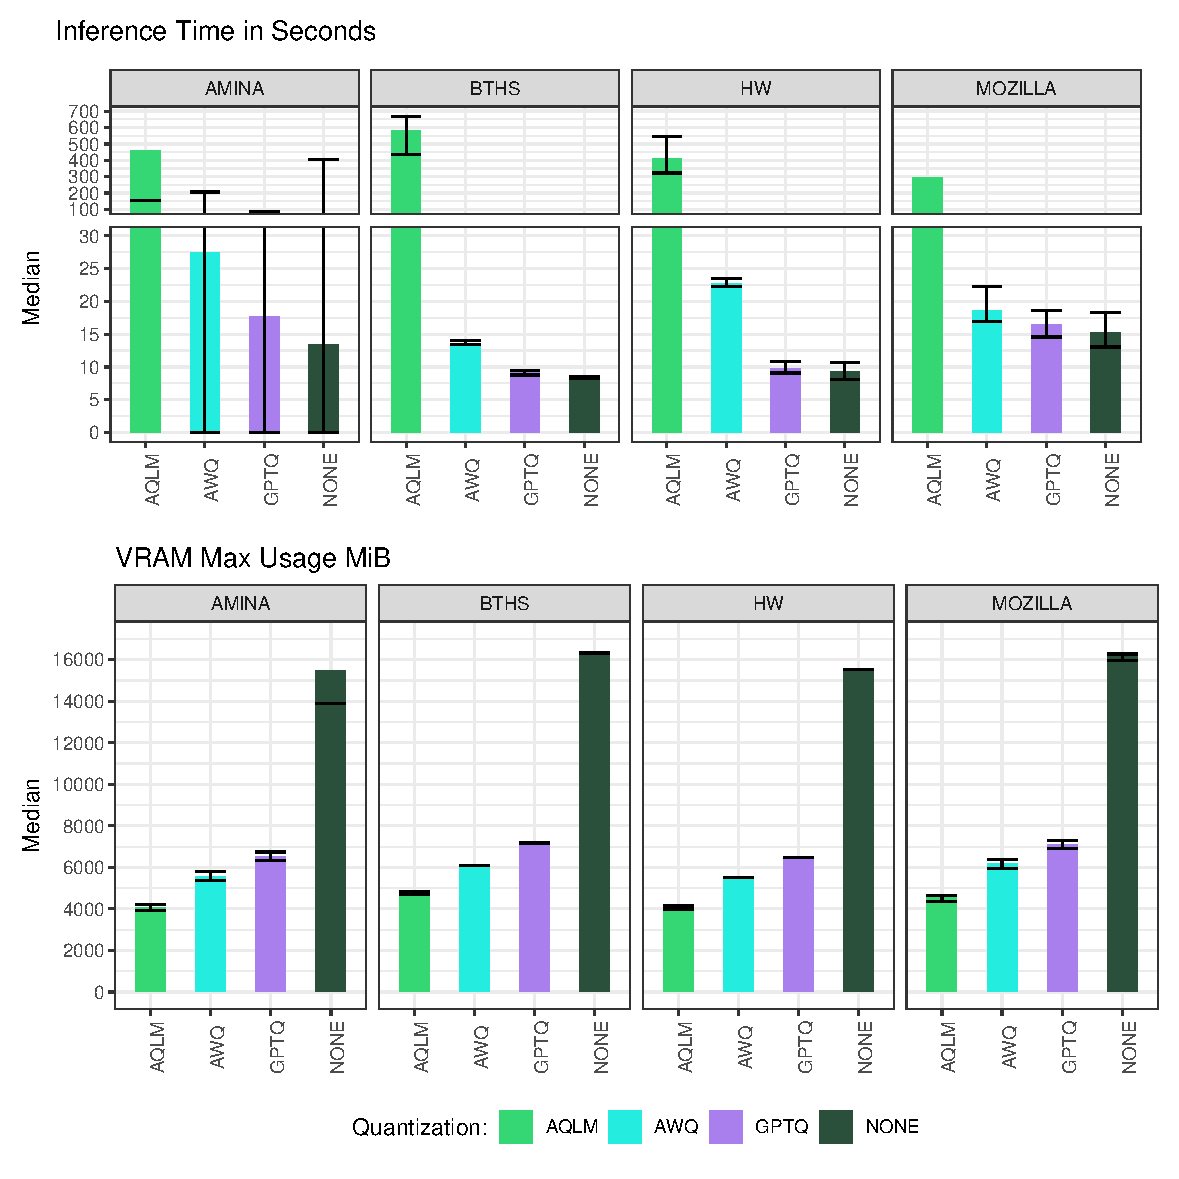
\includegraphics[width=0.8\textwidth]{images/RQ2.pdf}
    \caption{Treatment efficiency across the datasets}
    \label{fig:rq2}
\end{figure*}

We find that all quantization methods reduce VRAM usage by more than half in comparison to the full-precision model. Notably, AQLM reduces VRAM usage to a quarter of that required by the full-precision model. This can be verified in the Post-hoc table below, wherein AQLM receives a VDA score of $0.0$\footnote{In the context of RQ2, a low VDA score indicates that the model requires significantly \textit{fewer} resources compared to another treatment, meaning it is \textit{unlikely} to exceed the other model in that metric. This interpretation contrasts with the context of RQ1.} in every paired comparison with \textit{None}. 

The full-precision model achieves the fastest inference times compared to all quantized models, as shown in Figure~\ref{fig:rq2}, and this is evidenced by the high VDA scores. Notably, AQLM exhibits particularly high inference times. We frequently observed that AQLM would attempt to generate trace links indefinitely, likely due to its inability to properly interpret the context. This aligns with its poor performance discussed in the context of RQ1.

Secondly, AWQ requires on average the second lowest VRAM utilization, though in comparison to GPTQ---which may require some 1,000 MiB more---it takes on average almost as twice as long to perform inference (AWQ receives higher VDA scores in all its paired comparisons with GPTQ, an excerpt is highlighted in Table~\ref{tab:posthoc_mozilla}). However, from a practical perspective, this difference is negligible on datasets of this scale, see Figure~\ref{fig:rq2} below. 

\begin{table}[ht]
    \centering
    \caption{Post-hoc Analysis: Mozilla dataset}
    \resizebox{\linewidth}{!}{
    \begin{tabular}{llllrlr}
        \toprule
        Metric & Group $1$ & Group $2$ & $p$.adj & $p$.adj.signif & VDA & Magnitude\\
        \midrule
        Inference Time (s) & AQLM & NONE & 0.01 & Moderate & 1.00 & Large \\
        \rowcolor{hl_color_green}
        \phantom & AWQ & GPTQ & 0.01 & Moderate & 1.00 & Large \\
        \phantom & AWQ & NONE & 0.01 & Moderate & 1.00 & Large \\
        \phantom & GPTQ & NONE & 0.06 & Not significant & 0.90 & Large \\
        \midrule
        Maximum VRAM Usage (MiB) & AQLM & NONE & 0.02 & Moderate & 0.00 & Large \\
        \phantom & AWQ & NONE & 0.01 & Moderate & 0.00 & Large \\
        \phantom & AQLM & AWQ & 0.02 & Moderate & 0.00 & Large \\
        \phantom & AQLM & GPTQ & 0.01 & Moderate & 0.00 & Large \\
        \phantom & GPTQ & NONE & 0.02 & Moderate & 0.00 & Large \\
        \bottomrule
        \end{tabular}
    }
    \label{tab:posthoc_mozilla}
\end{table}

Lastly, the Mistral full-precision model has the highest memory consumption ranging up to 17,000 MiB of VRAM. Interestingly, it takes the least time to perform inference on average (whenever there is a pair model--\textit{None}, the expected VDA score for this pair is around $1$).

\textbf{Summary}: Quantized LLMs significantly reduce computational costs compared to full-precision models. Across all datasets, quantized models reduce VRAM usage by over 50\%, with GPTQ offering the best balance between memory efficiency and runtime speed---it retains a similar inference time than the one of base Mistral with a significant VRAM cut, as evidenced by Figure~\ref{fig:rq2} as well as the discussed VDA scores. Furthermore, it is worth noting that the results for VRAM in this table consistently show that quantized models outperform full-precision Mistral in every paired VDA comparison across all observations (see Appendix~\ref{app:posthoc_rq2}).

% deprecated -- too much clutter
% \begin{table}[ht]
\centering
\caption*{AMINA dataset}
\resizebox{\linewidth}{!}{
\begin{tabular}{llllrlr}
    \toprule
    Metric & Group $1$ & Group $2$ & $p$.adj & $p$.adj.signif & VDA & Magnitude\\
    \midrule
    Inference Time (s) & AQLM & NONE & 0.02 & Moderate & 0.90 & Large \\
    \rowcolor{hl_color_green}
    \phantom & AWQ & GPTQ & 0.25 & Not significant & 0.80 & Large \\
    \phantom & AWQ & NONE & 0.86 & Not significant & 0.80 & Large \\
    \phantom & GPTQ & NONE & 0.86 & Not significant & 0.80 & Large \\
    \midrule
    Maximum VRAM Usage (MiB) & AQLM & NONE & 0.02 & Moderate & 0.00 & Large \\
    \phantom & AQLM & AWQ & 0.01 & Moderate & 0.00 & Large \\
    \phantom & AQLM & GPTQ & 0.02 & Moderate & 0.00 & Large \\
    \phantom & AWQ & NONE & 0.02 & Moderate & 0.00 & Large \\
    \phantom & GPTQ & NONE & 0.02 & Moderate & 0.00 & Large \\
    \bottomrule
    \end{tabular}
}
\label{tab:RQ2_posthoc}
\end{table}

% \begin{table}[ht]
\centering
\caption*{BTHS dataset}
\resizebox{\linewidth}{!}{
    \begin{tabular}{llllrlr}
    \toprule
    Metric & Group $1$ & Group $2$ & $p$.adj & $p$.adj.signif & VDA & Magnitude\\
    \midrule
    Inference Time (s) & AQLM & AWQ & 0.01 & Moderate & 1.00 & Large \\
    \phantom & AQLM & GPTQ & 0.01 & Moderate & 1.00 & Large \\
    \phantom & AQLM & NONE & 0.01 & Moderate & 1.00 & Large \\
    \rowcolor{hl_color_green}
    \phantom & AWQ & GPTQ & 0.01 & Moderate & 1.00 & Large \\
    \phantom & AWQ & NONE & 0.01 & Moderate & 1.00 & Large \\
    \phantom & GPTQ & NONE & 0.01 & Moderate & 0.90 & Large \\
    \bottomrule
    \end{tabular}
}
\label{tab:RQ2_posthoc}
\end{table}

% \begin{table}[ht]
\centering
\caption*{Health Watcher dataset}
\resizebox{\linewidth}{!}{
    \begin{tabular}{llllrlr}
    \toprule
    Metric & Group $1$ & Group $2$ & $p$.adj & $p$.adj.signif & VDA & Magnitude\\
    \midrule
    Inference Time (s) & AQLM & AWQ & 0.01 & Moderate & 1.00 & Large \\
    \phantom & AQLM & GPTQ & 0.01 & Moderate & 1.00 & Large \\
    \phantom & AQLM & NONE & 0.01 & Moderate & 1.00 & Large \\
    \rowcolor{hl_color_green}
    \phantom & AWQ & GPTQ & 0.01 & Moderate & 1.00 & Large \\
    \phantom & AWQ & NONE & 0.01 & Moderate & 1.00 & Large \\
    \phantom & GPTQ & NONE & 0.49 & Not significant & 0.50 & Negligible \\
    \bottomrule
    \end{tabular}
}
\label{tab:RQ2_posthoc}
\end{table}


\subsection{\textbf{RQ3:} Models' Accuracy and Inference Time as Artifacts Increase}

We assess whether the costs associated with artifact size are significant enough to render REST alignment with LLMs infeasible in the long term. In many practical discussions, many might assume that inference time grows linearly with input size. However, our findings contradict this and it becomes evident that the inference time fits a sub-quadratic scale: specifically, a linearithmic scale (i.e., $n \log n$). This can be verified by running a linear regression algorithm\footnote{E.g. in Python \url{https://docs.scipy.org/doc/scipy/reference/generated/scipy.stats.linregress.html}} on the inference time data (see Appendix~\ref{app:supp-rq3}) which yields $R^2$ (coefficient of determination) scores for a linearithmic scale as suggesting a strong correlation in Table~\ref{tab:rsquared}.

\begin{table}[H]
    \centering
    \begin{tabular}{llc}
    \toprule
    \textbf{Model} & \textbf{Dataset} & \boldmath$R^2$ \\
    \midrule
    GPTQ & Mozilla & 0.9656 \\
    \textit{None}  & Mozilla & 0.9655 \\
    GPTQ & AMINA   & 0.9825 \\
    \textit{None}  & AMINA   & 0.9840 \\
    \bottomrule
    \end{tabular}
    \caption{$R^2$ for a linearithmic fit}
    \label{tab:rsquared}
\end{table}

The linearithmic increase is particularly related to the character distribution in the datasets and the nature of the prompt (cf. Table~\ref{tab:char_distribution}, Figure~\ref{fig:system_prompt}). For instance, the table suggests that on average, Mozilla consumes the most tokens on a prompt. Consequently, the inference time is higher than that of AMINA.

What is especially interesting is that the chosen quantization method is \textit{not} significantly advantageous to the base model here (in terms of the time inference), and the times almost overlap for each dataset. As suggested by \textbf{RQ2}, quantization helps to improve required compute resources, but our result shows that the artifact length still meaningfully affects inference time regardless of the quantization. This implies that the quantization does not change the scaling law in terms of input size. 

Interestingly, Figure~\ref{fig:RQ3_charts} confirms that severe degradation is seen for recall and $F_1$-scores as the sample size increases. This suggests that while the input size increases, more noise is introduced, and the models struggle to identify positives; this implies that the model becomes more ``conservative'' predicting fewer positives overall to avoid $FP$s, hence missing many $TP$s.

\begin{figure}[H]
    \centering
    \includesvg[width=0.85\columnwidth]{images/RQ3_excerpt.svg}
    \caption{Inference time \& chosen efficacy metrics against dataset subset size}
    \label{fig:RQ3_charts}
\end{figure}

Hence, we further address \textbf{RQ1} here, with findings that reinforce earlier results: GPTQ remains highly comparable to the full-precision model, occasionally outperforming it on key metrics---even as the sample size increases---supporting its viability as an alternative quantization method for REST efforts.

\begin{table*}[h!]
    \centering
    \begin{tabular}{p{3.5cm}p{4.5cm}p{7cm}}
    \toprule
    \textbf{Aspect} & \textbf{Observation} & \textbf{Implication} \\
    \midrule
    Inference time as input size grows & Linearithmic scale factor & Longer inputs lead to disproportionate increases in latency. \\
    \midrule
    Quantization & Remain stable \& almost identical throughout & The full-precision model and the top-performing quantized model (GPTQ) have almost identical observed efficacy, confirming quantization's viability. \\
    Accuracy \& Balanced Accuracy & Remain stable & Overall correctness preserved, but may mask other metric degradations. \\
    \midrule
    Precision & Mild degradation & This in turn yields an increase in $FP$s. \\
    \midrule
    Recall \& $F_1$-score & Severe degradation & Many $TP$s are missed on larger inputs; $F_1$-score drops sharply. \\
    \midrule
    Overall & Latency and performance degrade with larger input sizes regardless of quantization & Input size should be managed carefully for efficient, reliable performance. \\
    \bottomrule
    \end{tabular}
    \vspace{2mm} % nicely padded
    \caption{RQ3: Findings Summary}
    \label{tab:summary_findings}
\end{table*}

\textbf{Summary}: The inference time does not grow linearly and instead follows a linearithmic curve. Hence, practitioners should prioritize input truncation (e.g., removing duplicate or overlapping test cases) and summarization (e.g., reducing wordiness or overly specific descriptions) to minimize artifact (or sample) size, especially when low latency is critical and significant drops in recall or $F_1$-score are unacceptable. Furthermore, our findings reinforce the viability of quantization for REST traceability and provide additional support for the conclusions drawn in RQ2. Lastly, we prepare an overview of the discussed findings in Table~\ref{tab:summary_findings}.

\section{Discussion}

In this section, we delve into the implications of our findings and relate them to existing research. We aim to provide a comprehensive analysis of the contextual factors and challenges that influence and frame our findings. 

\subsection{Trade-offs of using quantized LLMs for REST}

All quantized models show significantly reduced VRAM usage, typically by up to $2.5$ times, compared to the full-precision Mistral model, which aligns with our hypothesis. While AQLM achieves the lowest VRAM usage due to aggressive quantization (2-bit width), it fails to adhere to the desired output format or simply gets stuck in a token-generation loop and is therefore not usable in practice for the purpose of REST alignment. 

We observed that the quantized models (AWQ and GPTQ) exhibited slower inference times compared to the full-precision model---which is an unexpected outcome, considering that we anticipated quantization to reduce inference time. We believe this is likely attributed to overhead that is incurred at runtime, such as the necessity to \textit{dequantize} (i.e., convert back to FP16) the quantized models for certain operations during inference. It is possible that the potential benefits of faster inference speeds are not realized when quantizing a relatively small LLM such as Mistral, and additional comparisons with larger models are needed for a conclusive answer. However, it is worth noting that while the results show a statistical significance in many cases, in practice, the difference is arguably negligible since all model treatments completed the task in less than 10 minutes. 

Among the quantized LLMs, GPTQ stands out as the most performant option, offering competitive results compared to the non-quantized model. AWQ has average results relative to full-precision Mistral and can serve as a somewhat reasonable alternative if GPTQ is unsuitable. Both GPTQ and AWQ demonstrate efficacy results that are comparable to, or even exceed, those of full-precision Mistral, indicating that quantized LLMs are a viable alternative for automated REST alignment.

The opportunity cost for LLMs (quantized or not) includes a dependence on GPU hardware as well as additional environment and/or container configuration in order to utilize the LLMs. As a consequence, this entails a relatively steep learning curve. In contrast, the Cosine Similarity algorithm is lightweight and hardly requires any hardware investments as it can run solely on a CPU, with an execution time of less than one second (in our observations). However, the need to pre-process the input data as well as fine-tune the threshold value on a subset of ground truth data increases its opportunity cost. The Cosine Similarity algorithm consistently demonstrates high prediction accuracy in the results. However, it is significantly constrained by language similarities in the input data, as it does not capture semantic meaning like LLMs do.

Yet, it is crucial to note that the performance results obtained in our experiment may not be broadly generalizable. Future experiments should explore additional configurations and a comprehensive evaluation under diverse conditions which include (but are not limited to) varied: hardware components, computing platforms, requirement and test datasets, and model selection. Here, we focus on specific configurations tailored for particular datasets and their properties to investigate initial gains and losses of quantized models.

Previous work by Quinstedt and Lindgren \cite{quinstedt2024Optimizing} has shown that LLMs with fewer parameters can perform comparably to larger models. In turn, our study demonstrates that quantized LLMs, smaller in terms of memory footprint, can achieve comparable, and in some cases superior, performance to their non-quantized counterparts. Furthermore, our results render successfully reduced memory usage which would be sufficient for (quantized) LLMs to run on a multitude of consumer-grade Nvidia GPUs.

However, RQ3 raises scalability concerns identified in earlier studies (e.g., \cite{ivarsson2023automated}). As previously discussed and in line with their work, our investigation into inference time suggests that the computational complexity may be linearithmic. However, this observation could be a result of our available datasets and their relatively small size; a larger dataset (e.g., thousands of requirements and tests; typically in complex systems) might possibly reveal behavior that tends toward polynomiality or even exponentiality. Notably, given the severe drop in efficacy metrics as artifact (input) size increases, additional sampling and/or processing techniques may be required to break down, categorize, and label data from such complex systems in a systematic way, which could further reinforce the viability of LLMs for REST alignment.

While achieving strict linearity may remain out of reach, further investigation is required to fully understand the correlation between dataset size and inference time. We ought to address current computational barriers with a focus on making LLM-aided REST alignment practical for use in complex systems.

\subsection{Challenges in adopting quantized LLMs}

While for this experiment we primarily used a cloud platform, the experiences we learned are still applicable when conducting a similar scenario for local use. Technology in LLMs is rapidly advancing, hence creating the need to keep up with frequent updates, whether in libraries, models, or other related dependencies. This can disrupt previously functioning code and configurations, resulting in additional costs and effort to keep existing implementations functioning and up-to-date.

As with both local and non-local usage, constantly evolving dependencies---often coupled with system-specific issues such as CUDA kernel configurations---can severely impact both development and usability. In our case, each quantized model required a separate environment and oftentimes an extensive setup effort. For example, setting up AQLM required provisioning a new Ubuntu-based container and presented numerous issues that were difficult to debug. Ultimately, the time and effort invested in this particular configuration were not justified by the unsatisfactory results discussed above.

Running models seamlessly on a standard developer machine remains a challenge. It is not uncommon to use non-Nvidia GPUs, especially Apple’s M-series chips, which are incompatible with Nvidia tools and require alternative solutions. Although Apple’s new Metal API offers some support, it is still maturing, and users continue to report integration issues. Still, for larger models like LLaMA and Mixtral, quantization alone may not reduce resource demands enough for smooth use without a high-end GPU. We experienced these limitations firsthand, even when running models on the Alvis cluster.

Moreover, we have also observed that despite having a well-defined prompt structure, not all quantized models adhere to these standards when providing response. For instance, AQLM repeatedly produced results in a practically unusable format. This discrepancy leads to additional parsing difficulties, increasing complexity and reducing the overall usability of such models.

Lastly, we have discovered that the size of the dataset significantly influences the performance of models. In particular, we have initially set up the experiment with the sample size of 100 entities. However, it was not feasible to run the entire experiment using the full data sets on other models (e.g., LLaMA 3, Mixtral). From the practical point of view, it appeared more realistic to proceed with data samples of 25 rows per document, which led to significantly better results.

\subsection{Choosing Between Cosine Similarity and LLMs}

The Cosine Similarity algorithm is a lightweight yet powerful solution when there is a substantial overlap in text among the files. However, it faces significant limitations with respect to semantic understanding. Based on our findings, we provide guidance on the scenarios in which this technique may be applicable.

\textbf{General recommendation:} Figure~\ref{fig:flowchart}  summarizes key considerations to help practitioners assess whether Cosine Similarity is an appropriate choice for their specific case. To make an informed decision, carefully review your data to identify if the requirement and test specification consistently use a set of keywords with little to no variations in phrasing. If this holds and you have ground truth annotations available to run a preliminary test of the algorithm, then it can serve as a light-weight solution to experiment with. Otherwise, consider using LLMs instead.

\begin{figure}[h]
    \centering
    \includesvg[width=0.8\columnwidth]{images/flowchart_upd.svg}
    \caption{Flowchart illustrating method selection guidelines}
    \label{fig:flowchart}
\end{figure}

\subsection{Questions for further research}

The implications of our study bring about some interesting research questions to further explore. Despite the resources challenges with the Alvis platform, we aim to extend this study in future work by introducing more quantization methods and datasets for evaluation. 

Further research should explore in-depth locally applied quantization of LLMs instead of relying on pre-quantized models available online; this can help to fully evaluate how quantized models compare to full-precision ones. Additionally, each quantization technique should be evaluated using multiple target bit-widths to investigate how the performance is affected by the increased information loss from more extreme target widths (and hence lowered maintenance expenses). Moreover, further investigation is needed into the feasibility of adjacent methods like Cosine Similarity in addition to heuristics from geometry, measure, and information theory, such as Minkowski distance, Haming Distance \cite{bookstein2002hammingdistance} Canberra and Chi-Square \cite{chi2005chisquare}, which are commonly used in machine learning to gauge similarity scores. Implementing one or an adapted combination of these techniques specifically for REST tasks could offer valuable insights. Exploring diverse approaches beyond the transformer-based LLMs encourages a broader perspective and increases the chances of identifying innovative and effective solutions.

Additionally, the LLMs used should be trained and/or fine-tuned specifically for the purposes of REST alignment (not just general-purpose models). This approach can help identify model configurations best suited for REST tasks. Since some quantization methods, notably AWQ, use input data during quantization to capture runtime activation ranges or prioritize important model components, this process can be tailored using fine-tuned REST data. This ensures activations reflect how the model behaves during REST alignment inference (i.e., trace link generation).

Lastly, more focus should be placed on scalability and the practicality of applying this approach to complex systems with thousands to tens of thousands requirements and tests---as is common in commercial settings. This may involve restructuring the evaluation pipeline to use more refined data formats or processing steps that reduce noise. For instance, adding a category attribute to test cases could allow filtering relevant subsets of requirements during evaluation. While this is just one of possibly many solutions, it highlights the need for investigating information management techniques to address the raised concerns of the approach.

\subsection{Threats to Validity}

Based on the guidelines proposed by Wohlin et al. \cite{wohlin2012experimentation} we identify the following threats to validity that might have influenced our research findings: 

\subsection*{\textbf{1) Internal Validity}}

\textit{Response variability}: due to the stochastic behavior of LLMs, the same prompt can result in different outputs when executed; we mitigate this risk by invoking prompts multiple times and defining consistent hyperparameters.

\textit{Selection of Models}: in this study, we select open-weight, state-of-the-art LLMs representative of a common choice among practitioners. This selection also leverages on the previous research by Quinstedt and Lindgren \cite{quinstedt2024Optimizing}. Aligning the selection of LLMs with their results allows for a more extensive and direct trade-off comparison. More models can be explored in future work, and we provide instrumentation in the Methodology section to facilitate smooth integration.

\textit{Quantized LLM Quality}: we have utilized quantized models distributed via the \textit{HuggingFace} platform. While all the quantization methods introduced in this study offer recommended implementation guidelines, the final results can still vary depending on how developers apply them during the quantization process. For example, quantization hyper-parameters (e.g., bit width, group size) and pre-processing steps (e.g., tokenization, weight normalization) can all significantly influence the performance of the quantized model. Although relying on third-party quantized models introduces some variability, HuggingFace remains one of the main sources for developers or organizations to download and/or deploy open weight models. As such, these models are likely to be used by practitioners, meaning that the results of our study are representative of the real-world use of quantized LLMs, given that this assumption holds.

\textit{Target Bit-widths}: Quantization techniques typically offer configurable target bit-widths to adjust the aggressiveness of the algorithm, influencing the amount of information lost from the original model. To comprehensively assess the impact of the selected quantization techniques it is necessary to explore several target bit-width levels for the models under test. However, due to scope limitations, this study focuses on a higher-level comparison of quantization techniques and does not encompass a broader range of target bit-widths. 

\subsection*{\textbf{2) External validity}}
    
\textit{Domain-Specific Applicability}: our study evaluates quantized LLMs within the specific use case of REST alignment. Exploring the trade-off of quantization in using LLMs for other Software Engineering tasks is beyond the scope of our thesis; however, it could be explored in future work.

\subsection*{\textbf{3) Construct validity}}

\textit{Ground Truth Validity}: the REST alignment mappings that are used in this study as ground truth were derived by employees at reputable industry companies and/or academic researchers. Although there is no guarantee of absolute correctness, the mappings reflect widely accepted data formats and standards in both industry and academic research.

\textit{Selection of Prompt Template}: the authors of the previous study that inspired our research questions explored different prompt templates and found that they can cause significant fluctuations in LLM output\cite{quinstedt2024Optimizing}. While it is possible that better prompt templates may exist, Quinstedt and Lindgren identified the most performant template, out of a set of templates, through a series of experiments \cite{quinstedt2024Optimizing}. Basing our template selection on their findings, derived in a similar context (automated REST alignment using LLMs), strengthens the credibility of our research.

\textit{Dependency Versioning}: because specific libraries sometimes require pinned versions of certain dependencies, we had to create an isolated environment for each quantization method we consider. As a result, central dependencies (e.g., \verb|torch|, \verb|transformers|, etc.) may be of different versions which may have a minimal impact on profiling, however, these dependencies typically differ by a few subversions, hence this risk is minimal. Furthermore, since the specified versions are necessary to run inference on certain quantized models, the potential impact versioning differences could have is representative of practical use of such models.

The Python (\verb|3.10.14|) and Conda (\verb|24.11.3|) versions remain unchanged as these, namely the version of the interpreter, have a direct impact on code execution speeds and therefore also on the benchmarking results.

\textit{Profiling -- Possible Overhead}: to time a certain code block, we rely on the \verb|perf_counter| function from Python's \verb|time| library. The function is specifically designed for measuring performance with the highest available resolution on a system-wide scale, hence making it an appropriate solution for benchmarking code segments and measuring execution time with microsecond precision.

To diminish any overhead in GPU metric retrieval, we rely on \verb|nvidia-smi| which provides an interface that can directly communicate with the hardware. It is worthwhile to mention that the tool comes with a negligible internal overhead, but from our possible options (provided by the Alvis platform) it is a well-established tool for profiling GPUs. 

We query metrics every 25 milliseconds to capture short-lived performance spikes—such as those occurring when initially loading a model. While this polling interval may not capture every event, it offers a practical balance between responsiveness and system overhead. Despite this, minor variations across repeated runs are expected due to caching and system-level effects. However, we mitigate these effects by reloading the model between every repetition of the experiment. 

\section*{Conclusion}

Our research highlights that quantized LLMs serve as an effective solution to reduce hardware overhead, and we conclude that quantized LLMs show promise in terms of automating REST alignment since certain quantization techniques either match or even exceed the performance of the full-precision model in our study.

There is, however, still areas to explore in terms of actively fine-tuning LLMs for REST alignment purposes, both during initial training (comparatively harder due to immense resource costs) and during the quantization process (cheaper and more feasible) by using input data that is similar to the target use and context. Additionally, our pilot study consisting of the Cosine Similarity baseline solution revealed a potential of possible adjacent strategies that could support REST tasks. Future research should explore additional heuristics and approaches in an inter-disciplinary manner, combining known strategies from various branches of mathematics or information science to further assist in REST alignment efforts---all of which warrants additional attention.

Despite the resource constraints and challenges encountered on the Alvis platform, we aim to extend this study in future work by evaluating a broader range of models, including state-of-the-art architectures like DeepSeek, and potentially explore other emerging quantization methods.

Lastly, more emphasis should be placed on the writing of requirements and test case descriptions. As demonstrated in this study (RQ3), excessive text has a detrimental impact on performance, and efficacy is similarly reduced due to noise and unnecessarily wordy phrasing. Clear and concise REST specifications are a useful blueprint to improve alignment efforts beyond the technical elements.

\section*{Acknowledgment}

We dedicate our gratitude to our supervisor Francisco Gomes de Oliveira Neto and our examiner Jennifer Horkoff for their valuable insights and continuous support. Furthermore, we are thankful for being able to use the computing platform---Alvis---offered by the Chalmers Centre for Computational Science and Engineering.

\bibliographystyle{IEEEtran}
\bibliography{lib}

% Appendix env.
\newcounter{appendixctr}

\newcommand{\Appendix}[2]{%
  \refstepcounter{appendixctr}%
  \section*{Appendix~\Roman{appendixctr}: #1}%
  \label{#2}%
  \addcontentsline{toc}{section}{Appendix~\Roman{appendixctr}: #1}%
}

\makeatletter
\renewcommand{\p@appendixctr}{}
\makeatother

\onecolumn

\Appendix{Datasets}{app:datasets}

\begin{table}[h]
  \centering
  \caption{Dataset specification: BTHS \& HealthWatcher}
  \begin{tabular}{lcccccccccc}
  \toprule
  Dataset & RE & ST & Pos. & Neg. & Prevalence ($\%$) & $1{:}1$ & $1{:}M$ & $M{:}1$ & $N{:}M$ & Unassigned \\
  \midrule
  BTHS           & 8 & 15 & 20 & 100 & 16.67 & 1:1 & 3:8 & 0:0 & 3:6 & 1\\
  HealthWatcher & 9 & 9 & 9 & 72 & 11.11 & 9:9 & 0:0 & 0:0 & 0:0 & 0\\
  \bottomrule
  \end{tabular}
  \label{tab:bths-hw}
\end{table}

\begin{table}[h]
  \centering
  \caption{Dataset specification: AMINA ($\text{sample}=25$)}
  \begin{tabular}{lcccccccccc}
  \toprule
  Sample & RE & ST & Pos. & Neg. & Prevalence ($\%$) & $1{:}1$ & $1{:}M$ & $M{:}1$ & $N{:}M$ & Unassigned \\
  \midrule
    01 & 25 & 40 & 41 & 959 & 4.1 & 18:18 & 5:20 & 1:1 & 1:2 & 0\\
    02 & 25 & 31 & 31 & 744 & 4.0 & 19:19 & 6:12 & 0:0 & 0:0 & 0\\
    03 & 25 & 38 & 39 & 911 & 4.11 & 19:19 & 4:17 & 1:1 & 1:2 & 0\\
    04 & 25 & 31 & 31 & 744 & 4.0 & 20:20 & 5:11 & 0:0 & 0:0 & 0\\
    05 & 25 & 31 & 31 & 744 & 4.0 & 20:20 & 5:11 & 0:0 & 0:0 & 0\\
    06 & 25 & 30 & 30 & 720 & 4.0 & 21:21 & 4:9 & 0:0 & 0:0 & 0\\
    07 & 25 & 37 & 37 & 888 & 4.0 & 22:22 & 3:15 & 0:0 & 0:0 & 0\\
    08 & 25 & 39 & 39 & 936 & 4.0 & 20:20 & 5:19 & 0:0 & 0:0 & 0\\
    09 & 25 & 30 & 31 & 719 & 4.13 & 19:19 & 4:9 & 1:1 & 1:2 & 0\\
    10 & 25 & 32 & 32 & 768 & 4.0 & 18:18 & 7:14 & 0:0 & 0:0 & 0\\
  \bottomrule
  \end{tabular}
  \label{tab:amina}
\end{table}

\begin{table}[h]
  \centering
  \caption{Dataset specification: Mozilla ($\text{sample}=25$)}
  \begin{tabular}{lcccccccccc}
  \toprule
  Sample & RE & ST & Pos. & Neg. & Prevalence ($\%$) & $1{:}1$ & $1{:}M$ & $M{:}1$ & $N{:}M$ & Unassigned \\
  \midrule
  	01 & 25 & 25 & 25 & 600 & 4.0 & 25:25 & 0:0 & 0:0 & 0:0 & 0\\
	02 & 25 & 21 & 21 & 504 & 4.0 & 21:21 & 0:0 & 0:0 & 0:0 & 4\\
	03 & 25 & 20 & 20 & 480 & 4.0 & 20:20 & 0:0 & 0:0 & 0:0 & 5\\
	04 & 25 & 20 & 20 & 480 & 4.0 & 20:20 & 0:0 & 0:0 & 0:0 & 5\\
	05 & 25 & 23 & 23 & 552 & 4.0 & 23:23 & 0:0 & 0:0 & 0:0 & 2\\
	06 & 25 & 23 & 23 & 552 & 4.0 & 23:23 & 0:0 & 0:0 & 0:0 & 2\\
	07 & 25 & 22 & 22 & 528 & 4.0 & 22:22 & 0:0 & 0:0 & 0:0 & 3\\
	08 & 25 & 21 & 21 & 504 & 4.0 & 21:21 & 0:0 & 0:0 & 0:0 & 4\\
	09 & 25 & 18 & 18 & 432 & 4.0 & 18:18 & 0:0 & 0:0 & 0:0 & 7\\
	10 & 25 & 19 & 19 & 456 & 4.0 & 19:19 & 0:0 & 0:0 & 0:0 & 6\\
  \bottomrule
  \end{tabular}
  \label{tab:mozilla}
\end{table}

\begin{table}[h]
    \centering
    \caption{Full dataset character distribution}
    \begin{tabular}{lllccccc}
    \toprule
    Dataset & RE & ST & Feature & Description & Purpose & Test steps & Prompt* \\
    \midrule
    AMINA         & 100 & 130 & 27.54 & 153.32 & 32.59  & 172.12 & 6,291  \\
    BTHS          & 8 & 15    & 33.75 & 487.50 & 103.67 & 677.80 & 13,235 \\
    Mozilla       & 316 & 254 & 18.92 & 81.41  & 103.34 & 663.65 & 20,268 \\
    HealthWatcher & 9 & 9     & 16.89 & 177.44 & 0      & 996.78 & 10,157  \\
    \bottomrule
    \end{tabular}
    \label{tab:char_distribution}
\end{table}

*For each dataset, the average prompt string length is calculated as: fixed prompt template length $+$ average requirement string length $+$ (number of tests $\times$ average test string length).

\newpage
\Appendix{Dataset Examples}{app:dataset_examples}

\hspace{1.5em}\textbf{AMINA}
\begin{roundedBox-sm}
    \textbf{RE:} B62, Energy values to other system within 10 sec, The energy values (15-minute values) shall be exportable from HES via integrations to other systems within 10 seconds after registration in HES.
    \\[0.5em]
    \textbf{ST:} 194, Energy values to other system within 10 sec, Verify that the goods are delivered from HES according to the agreed export interval
    \\[0.5em]
   \textbf{Mapping:} B62,194
\end{roundedBox-sm}

 \begin{roundedBox-sm}
    \textbf{RE:} B107,Version control of web service interfaces,Web service interfaces should (B107) be version controlled so that old versions can be used if necessary.
    \\[0.5em]
    \textbf{ST:} 25,Version control of web service interfaces,Verify that the previous version of the web service interface can be read back and is compatible with the new version or previous version of ACM.
    \\[0.5em]
    \textbf{Mapping:} B107,25
\end{roundedBox-sm}

\hspace{1.5em}\textbf{BTHS}
\begin{roundedBox-sm}
    \textbf{RE:} 4.6.1,Audio Connection Transfer from AG to HS,"The audio connection transfer from AG to HS is initiated by a user action on the HS side. To effect this transfer, the HS shall send the AT+CKPD=200 command to the AG."
    \\[0.5em]
    \textbf{Tests:} HSP/AG/ACT/BV-01-I,"To verify that the AG can perform an audio connection transfer from AG to HS initiated by a user
action on the headset.","Initial condition: 
- Both devices are initilized. Ensure HS and AG are initially paired, confirming interoperability for the headset profile. 
- HS is in Standby mode, no connection to AG
- For AG a call/audio connection is active at the AG.

Procedure: 
HS: Initiate the user action (e.g. press button) on the HS to transfer the audio connection from AG to HS
AG:No user action is required
  
Expected Outcome AG:The user action on the HS transfers the audio connection from AG to HS"
    \\[0.5em]
    \textbf{Mapping:} 4.6.1,HSP/AG/ACT/BV-01-I
\end{roundedBox-sm}

\hspace{1.5em}\textbf{HealthWatcher}
\begin{roundedBox-sm}
    \textbf{RE:} FR15,Update health unit,This use case allows the health unit's data to be updated.
    \\[0.5em]
    \textbf{ST:} T-8,,"1. The employee chooses the update health unit option.
2. The system retrieves the list of all health units.
3. The list of health units is returned to the employee.
4. The list of health units is formatted and displayed on the employee’s local display.
5. The employee selects the health unit to be updated.
6. The unique identifier for the selected health unit is sent to the server.
7. The system ensures the health unit data is consistent.
8. The system retrieves the data for the selected health unit.
9. The data retrieved is returned to the employee.
10.The health unit data is formatted and presented on the employee’s local display.
11.The employee alters the necessary data.
12.The updated information is sent to the server.
13.The system ensures the health unit data is left in a consistent state. 
14.The system stores the updated health unit information."
    \\[0.5em]
    \textbf{Mapping:} FR15,T-8
\end{roundedBox-sm}

\hspace{1.5em}\textbf{Mozilla}

\begin{roundedBox-sm}
    \textbf{RE:} R-005,Double-clicking on a bookmark shall cause it to be launched in a browser window.,Double-clicking on a bookmark shall cause it to be launched in a browser window.
    \\[0.5em]
    \textbf{ST:}
    TC-005,,"INITIAL CONDITIONS
    1. You must have a bookmarks file.
    2. To promote consistency, you may choose to use the default set of Netscape Seamonkey Bookmarks.
    3. You also have the option to use this very large bookmarks file.
    4. You must also customize your sidebar to include a bookmarks panel.
    
    STEPS/DESCRIPTION
    1. Select the toplevel ""Bookmarks"" menu. Select any bookmark on the list.
    2. Click ""Bookmarks"" on the Bookmarks/personal toolbar. Select any bookmark on the list.
    3. Open the sidebar; click on the ""Bookmarks"" panel. Double-click any bookmark on the list.
    4. From the toplevel ""Bookmarks"" menu select ""Manage Bookmarks"". Double-click any bookmark in the window.
    
    EXPECTED RESULTS
    In all cases, the url corresponding to the bookmark you selected should be loaded in the browser window.
    
    LINKS
    1. default-bookmarks.html
    2. large-bookmarks.html"
    \\[0.5em]
    \textbf{Mapping:} R-005,TC-005
\end{roundedBox-sm}

\newpage % break
\Appendix{Cosine Similarity Pilot Study}{app:cosine}

We conducted a pilot study, experimenting with different threshold values for the Cosine Similarity algorithm. As a starting point, we executed the Cosine Similarity algorithm independently on the Mozilla dataset with the following randomly selected thresholds: 0.14, 0.24 and 0.34. We considered threshold values below 0.5 as the requirements and tests in consideration are expected to showcase moderate similarities, yet have inherent differences in their content. Higher thresholds risk missing relevant links by making the algorithm overly conservative in its matching. Therefore, we partition the interval of $[0, 0.5]$ into roughly equivalent segments for evaluation. When evaluating LLMs, we utilize subsets for the larger datasets (such as Mozilla), thus we apply the same principle in this step as well. We compute balanced accuracy, precision, recall, accuracy, and $F_1$-score metrics for the Mozilla dataset as a representative sample dataset, see results in Table~\ref{tab:performance_metrics} below.

\begin{table}[h!]
\centering
\caption{Mozilla dataset performance metrics at different threshold values}
\begin{tabular}{lcccccccccc}
    \toprule
    Threshold & Accuracy & Balanced Accuracy & Precision & Recall & $F_1$-score & TP & FP & TN & FN \\
    \midrule
    0.14 & 0.9486 & 0.7214 & 0.4467 & 0.9092 & 0.5930 & 193 & 257 & 4831 & 19  \\
    0.24 & 0.9689 & 0.7937 & 0.5947 & 0.8280 & 0.6833 & 176 & 129 & 4959 & 36  \\
    0.34 & 0.9770 & 0.8505 & 0.7116 & 0.7441 & 0.7217 & 158 & 68  & 5020 & 54  \\
    \bottomrule
\end{tabular}
\label{tab:performance_metrics}
\end{table}

When analyzing the obtained results, we prioritize $F_1$-score as the primary selection criterion because it provides a balanced measure of precision and recall. Next, we consider high recall to ensure that relevant instances are not missed, and lastly evaluate the precision in its capacity to reduce false positives. We conclude that the threshold with value 0.34 yielded the most favorable results. The observed $F_1$-score with the value 0.72 and harmonic combination of recall (0.74) and precision (0.71) indicate that this is an optimal threshold. As a result, we select this value and consistently use it to execute the Cosine Similarity script with the rest of the datasets. 
Please find the distribution of the evaluation metric values for each dataset below:

\begin{table}[h!]
    \centering
    \caption{Performance metrics across different datasets with threshold $0.34$}
    \begin{tabular}{lcccccccccc}
    \toprule
    Dataset & Accuracy & Balanced Accuracy & Precision & Recall & $F_1$-score & TP & FP & TN & FN \\
    \midrule
    AMINA & 0.9889 & 0.9604 & 0.9295 & 0.7890 & 0.8485 & 266 & 21  & 8112 & 76  \\
    BTHS & 0.7833 & 0.6556 & 0.4000 & 0.6000 & 0.4800 & 120 & 180 & 820  & 80  \\
    Mozilla & 0.9770 & 0.8505 & 0.7116 & 0.7441 & 0.7217 & 158 & 68  & 5020 & 54  \\
    HealthWatcher & 0.8889 & 0.7218 & 0.5000 & 0.5556 & 0.5263 & 50  & 50  & 670  & 40  \\
    \bottomrule
    \end{tabular}
    \label{tab:dataset_performance}
\end{table}

\newpage
\Appendix{Analysis Supplementary Material: Box plots}{app:boxplots}

\begin{figure}[ht]
    \centering
    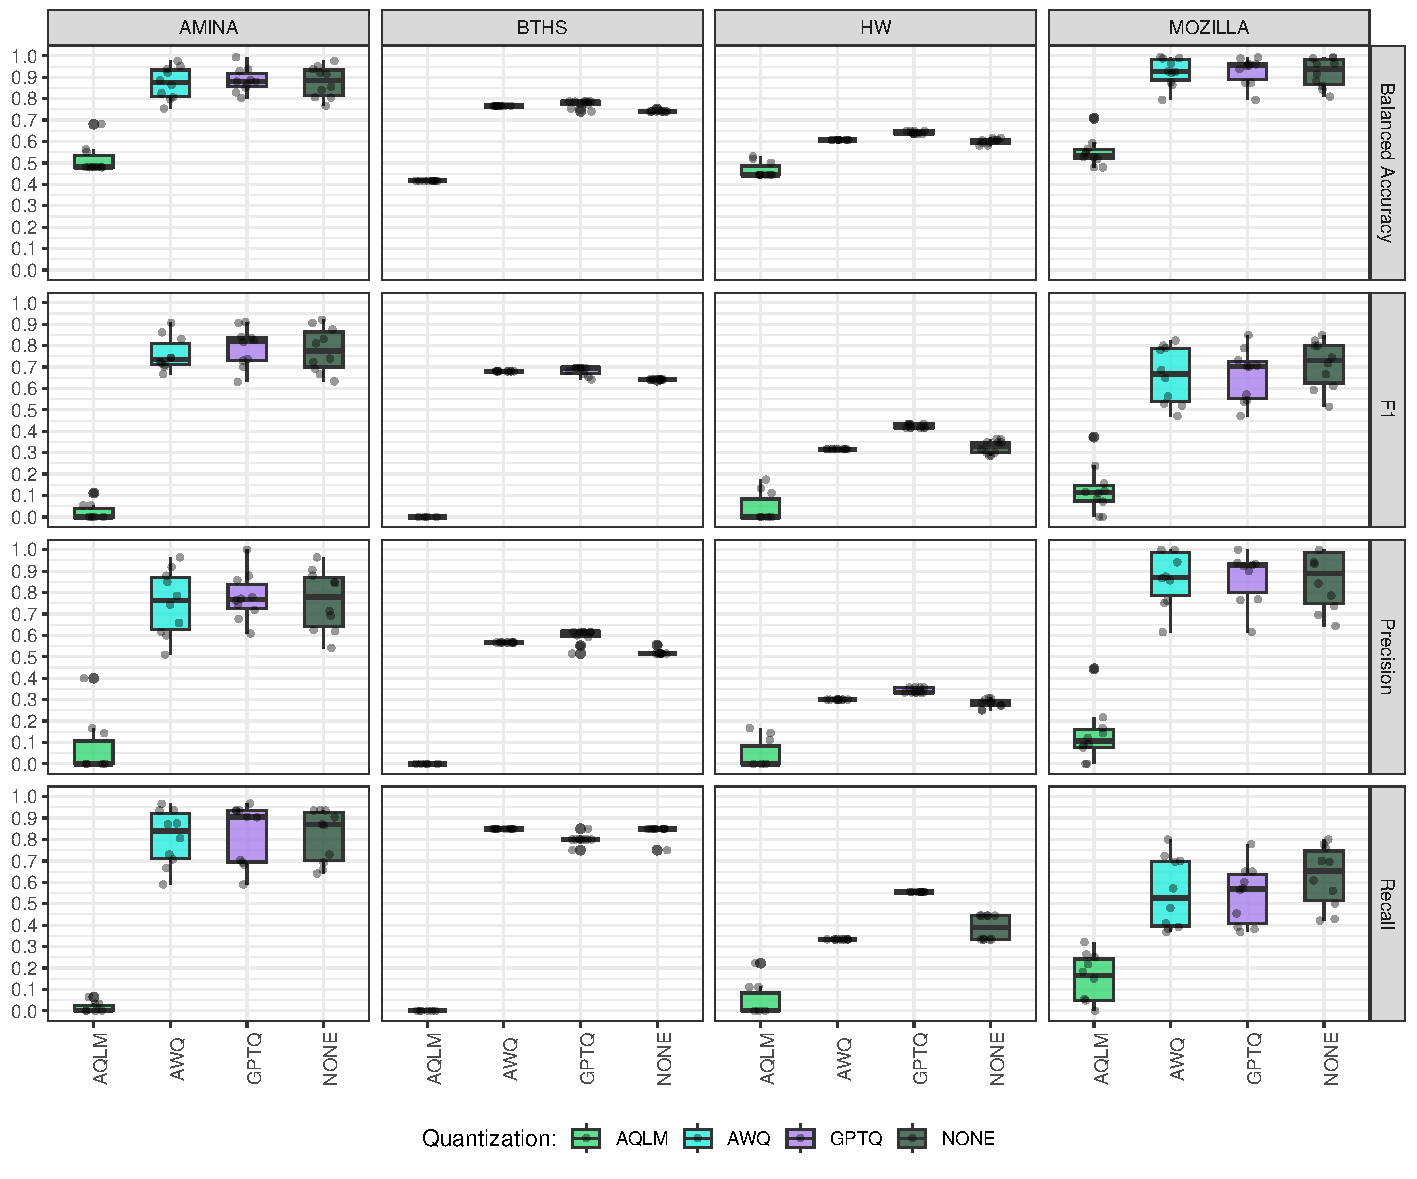
\includegraphics[width=0.95\textwidth]{images/RQ1_box_plot.pdf}
    \caption{Efficacy across the datasets}
    \label{fig:RQ1_boxplot_full}
\end{figure}

\begin{figure}[ht]
    \centering
    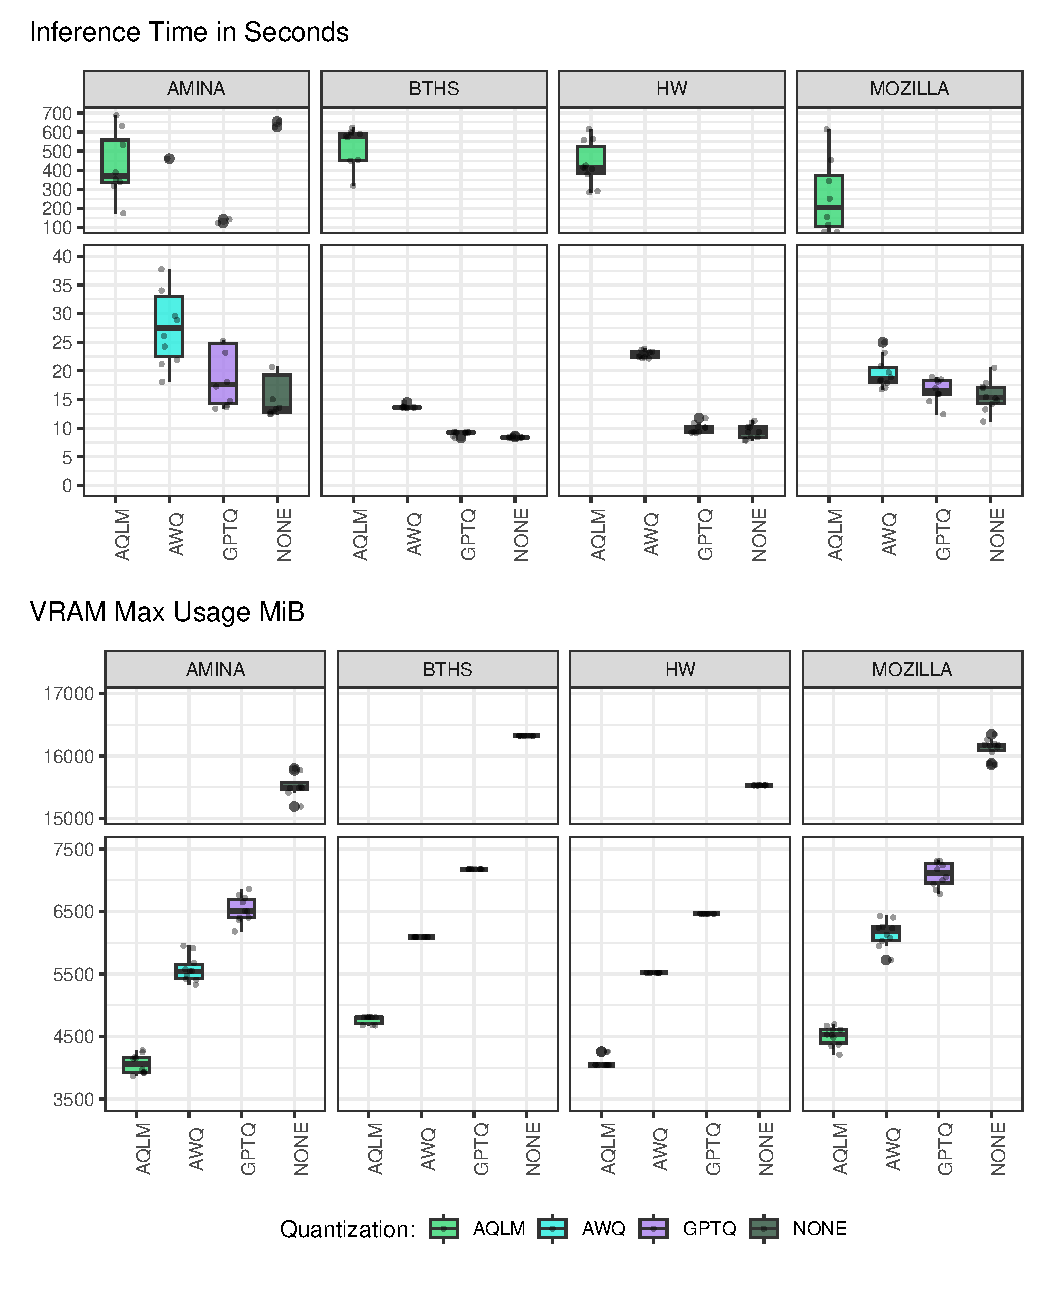
\includegraphics[width=0.85\textwidth]{images/RQ2_box_plot.pdf}
    \caption{Efficiency accross the datasets}
    \label{fig:RQ2_boxplot_full}
\end{figure}

\newpage
\Appendix{Post-hoc Results for RQ1}{app:posthoc_rq1}

\begin{table}[H]
\centering
\caption*{AMINA dataset}
\begin{tabular}{llllllrlr}
\toprule
Metric & Group $1$ & Group $2$ & Statistic & $p$ & $p$.adj & $p$.adj.signif & VDA & Magnitude\\
\midrule
Balanced accuracy & AQLM & AWQ & 0 & 0.012 & 0.01 & Moderate & 0.00 & Large \\
\phantom & AQLM & GPTQ & 0 & 0.012 & 0.01 & Moderate & 0.00 & Large \\
\phantom & AQLM & NONE & 0 & 0.012 & 0.01 & Moderate & 0.00 & Large \\
\phantom & AWQ & GPTQ & 20 & 1.000 & 1.00 & Not significant & 0.40 & Small \\
\phantom & AWQ & NONE & 17 & 1.000 & 1.00 & Not significant & 0.50 & Negligible \\
\phantom & GPTQ & NONE & 32 & 1.000 & 1.00 & Not significant & 0.50 & Negligible \\
\midrule
Recall & AQLM & AWQ & 0 & 0.012 & 0.01 & Moderate & 0.00 & Large \\
\phantom & AQLM & GPTQ & 0 & 0.024 & 0.02 & Moderate & 0.00 & Large \\
\phantom & AQLM & NONE & 0 & 0.012 & 0.01 & Moderate & 0.00 & Large \\
\phantom & AWQ & GPTQ & 10 & 0.882 & 0.88 & Not significant & 0.40 & Small \\
\phantom & AWQ & NONE & 13 & 0.882 & 0.88 & Not significant & 0.40 & Small \\
\phantom & GPTQ & NONE & 24 & 0.882 & 0.88 & Not significant & 0.60 & Small \\
\midrule
Precision & AQLM & AWQ & 0 & 0.012 & 0.01 & Moderate & 0.00 & Large \\
\phantom & AQLM & GPTQ & 0 & 0.012 & 0.01 & Moderate & 0.00 & Large \\
\phantom & AQLM & NONE & 0 & 0.012 & 0.01 & Moderate & 0.00 & Large \\
\phantom & AWQ & GPTQ & 20 & 1.000 & 1.00 & Not significant & 0.40 & Small \\
\phantom & AWQ & NONE & 17 & 1.000 & 1.00 & Not significant & 0.50 & Negligible \\
\phantom & GPTQ & NONE & 32 & 1.000 & 1.00 & Not significant & 0.50 & Negligible \\
\midrule
$F_1$-score & AQLM & AWQ & 0 & 0.012 & 0.01 & Moderate & 0.00 & Large \\
\phantom & AQLM & GPTQ & 0 & 0.012 & 0.01 & Moderate & 0.00 & Large \\
\phantom & AQLM & NONE & 0 & 0.012 & 0.01 & Moderate & 0.00 & Large \\
\phantom & AWQ & GPTQ & 18 & 1.000 & 1.00 & Not significant & 0.40 & Small \\
\phantom & AWQ & NONE & 17 & 1.000 & 1.00 & Not significant & 0.60 & Small \\
\phantom & GPTQ & NONE & 30 & 1.000 & 1.00 & Not significant & 0.50 & Negligible \\\end{tabular}
\label{tab:RQ1_posthoc_full}
\end{table}

\begin{table}[h]
\centering
\caption*{HealthWatcher dataset}
\begin{tabular}{llllllrlr}
\toprule
Metric & Group $1$ & Group $2$ & Statistic & $p$ & $p$.adj & $p$.adj.signif & VDA & Magnitude\\
\midrule
Balanced accuracy & AQLM & GPTQ & 0 & 0.016 & 0.02 & Moderate & 0.00 & Large \\
\phantom & AQLM & NONE & 0 & 0.016 & 0.02 & Moderate & 0.00 & Large \\
\phantom & GPTQ & NONE & 55 & 0.016 & 0.02 & Moderate & 1.00 & Large \\
\midrule
Recall & AQLM & NONE & 0 & 0.004 & 0.00 & Strong & 0.00 & Large \\
\midrule
Precision & AQLM & GPTQ & 0 & 0.016 & 0.02 & Moderate & 0.00 & Large \\
\phantom & AQLM & NONE & 0 & 0.016 & 0.02 & Moderate & 0.00 & Large \\
\phantom & GPTQ & NONE & 55 & 0.016 & 0.02 & Moderate & 1.00 & Large \\
\midrule
$F_1$-score & AQLM & GPTQ & 0 & 0.016 & 0.02 & Moderate & 0.00 & Large \\
\phantom & AQLM & NONE & 0 & 0.016 & 0.02 & Moderate & 0.00 & Large \\
\phantom & GPTQ & NONE & 55 & 0.016 & 0.02 & Moderate & 1.00 & Large \\\end{tabular}
\label{tab:RQ1_posthoc_full}
\end{table}

\begin{table}[ht]
\centering
\caption*{BTHS dataset}
\begin{tabular}{llllllrlr}
\toprule
Metric & Group $1$ & Group $2$ & Statistic & $p$ & $p$.adj & $p$.adj.signif & VDA & Magnitude\\
\midrule
Balanced accuracy & GPTQ & NONE & 45 & 0.008 & 0.01 & Strong & 0.95 & Large \\
\midrule
Recall & GPTQ & NONE & 8 & 0.081 & 0.08 & Not significant & 0.15 & Large \\
\midrule
Precision & GPTQ & NONE & 45 & 0.008 & 0.01 & Strong & 0.95 & Large \\
\midrule
$F_1$-score & GPTQ & NONE & 45 & 0.008 & 0.01 & Strong & 0.95 & Large \\\end{tabular}
\label{tab:RQ1_posthoc_full}
\end{table}

\begin{table}[h]
\centering
\caption*{Mozilla dataset}
\begin{tabular}{llllllrlr}
\toprule
Metric & Group $1$ & Group $2$ & Statistic & $p$ & $p$.adj & $p$.adj.signif & VDA & Magnitude\\
\midrule
Balanced accuracy & AQLM & AWQ & 0 & 0.012 & 0.01 & Moderate & 0.00 & Large \\
\phantom & AQLM & GPTQ & 0 & 0.012 & 0.01 & Moderate & 0.00 & Large \\
\phantom & AQLM & NONE & 0 & 0.012 & 0.01 & Moderate & 0.00 & Large \\
\phantom & AWQ & GPTQ & 19 & 1.000 & 1.00 & Not significant & 0.55 & Negligible \\
\phantom & AWQ & NONE & 15 & 1.000 & 1.00 & Not significant & 0.40 & Small \\
\phantom & GPTQ & NONE & 24 & 1.000 & 1.00 & Not significant & 0.35 & Small \\
\midrule
Recall & AQLM & AWQ & 0 & 0.012 & 0.01 & Moderate & 0.00 & Large \\
\phantom & AQLM & GPTQ & 0 & 0.012 & 0.01 & Moderate & 0.00 & Large \\
\phantom & AQLM & NONE & 0 & 0.012 & 0.01 & Moderate & 0.00 & Large \\
\phantom & AWQ & GPTQ & 13 & 0.675 & 0.68 & Not significant & 0.50 & Negligible \\
\phantom & AWQ & NONE & 0 & 0.045 & 0.04 & Moderate & 0.15 & Large \\
\phantom & GPTQ & NONE & 1 & 0.039 & 0.04 & Moderate & 0.15 & Large \\
\midrule
Precision & AQLM & AWQ & 0 & 0.012 & 0.01 & Moderate & 0.00 & Large \\
\phantom & AQLM & GPTQ & 0 & 0.012 & 0.01 & Moderate & 0.00 & Large \\
\phantom & AQLM & NONE & 0 & 0.012 & 0.01 & Moderate & 0.00 & Large \\
\phantom & AWQ & GPTQ & 13 & 1.000 & 1.00 & Not significant & 0.40 & Small \\
\phantom & AWQ & NONE & 12 & 1.000 & 1.00 & Not significant & 0.45 & Negligible \\
\phantom & GPTQ & NONE & 18 & 1.000 & 1.00 & Not significant & 0.45 & Negligible \\
\midrule
$F_1$-score & AQLM & AWQ & 0 & 0.012 & 0.01 & Moderate & 0.00 & Large \\
\phantom & AQLM & GPTQ & 0 & 0.012 & 0.01 & Moderate & 0.00 & Large \\
\phantom & AQLM & NONE & 0 & 0.012 & 0.01 & Moderate & 0.00 & Large \\
\phantom & AWQ & GPTQ & 21 & 0.906 & 0.91 & Not significant & 0.45 & Negligible \\
\phantom & AWQ & NONE & 1 & 0.042 & 0.04 & Moderate & 0.20 & Large \\
\phantom & GPTQ & NONE & 1 & 0.039 & 0.04 & Moderate & 0.15 & Large \\\end{tabular}
\label{tab:RQ1_posthoc_full}
\end{table}


\Appendix{Post-hoc Results for RQ2}{app:posthoc_rq2}

\begin{table}[H]
\centering
\caption*{AMINA dataset}
\begin{tabular}{llllllrlr}
\toprule
Metric & Group $1$ & Group $2$ & Statistic & $p$ & $p$.adj & $p$.adj.signif & VDA & Magnitude\\
\midrule
Inference Time (s) & AQLM & AWQ & 55 & 0.012 & 0.01 & Moderate & 1.00 & Large \\
\phantom & AQLM & GPTQ & 55 & 0.012 & 0.01 & Moderate & 1.00 & Large \\
\phantom & AQLM & NONE & 53 & 0.023 & 0.02 & Moderate & 0.90 & Large \\
\phantom & AWQ & GPTQ & 45 & 0.252 & 0.25 & Not significant & 0.80 & Large \\
\phantom & AWQ & NONE & 36 & 0.864 & 0.86 & Not significant & 0.80 & Large \\
\phantom & GPTQ & NONE & 36 & 0.864 & 0.86 & Not significant & 0.80 & Large \\
\midrule
Maximum VRAM Usage (MiB) & AQLM & AWQ & 0 & 0.012 & 0.01 & Moderate & 0.00 & Large \\
\phantom & AQLM & GPTQ & 0 & 0.024 & 0.02 & Moderate & 0.00 & Large \\
\phantom & AQLM & NONE & 0 & 0.024 & 0.02 & Moderate & 0.00 & Large \\
\phantom & AWQ & GPTQ & 0 & 0.012 & 0.01 & Moderate & 0.00 & Large \\
\phantom & AWQ & NONE & 0 & 0.024 & 0.02 & Moderate & 0.00 & Large \\
\phantom & GPTQ & NONE & 0 & 0.024 & 0.02 & Moderate & 0.00 & Large \\
\bottomrule
\end{tabular}
\label{tab:RQ2_posthoc_full}
\end{table}

\begin{table}[ht]
\centering
\caption*{HealthWatcher dataset}
\begin{tabular}{llllllrlr}
\toprule
Metric & Group $1$ & Group $2$ & Statistic & $p$ & $p$.adj & $p$.adj.signif & VDA & Magnitude\\
\midrule
Inference Time (s) & AQLM & AWQ & 55 & 0.012 & 0.01 & Moderate & 1.00 & Large \\
\phantom & AQLM & GPTQ & 55 & 0.012 & 0.01 & Moderate & 1.00 & Large \\
\phantom & AQLM & NONE & 55 & 0.012 & 0.01 & Moderate & 1.00 & Large \\
\phantom & AWQ & GPTQ & 55 & 0.012 & 0.01 & Moderate & 1.00 & Large \\
\phantom & AWQ & NONE & 55 & 0.012 & 0.01 & Moderate & 1.00 & Large \\
\phantom & GPTQ & NONE & 35 & 0.492 & 0.49 & Not significant & 0.50 & Negligible \\
\bottomrule
\end{tabular}
\label{tab:RQ2_posthoc_full}
\end{table}

\begin{table}[ht]
\centering
\caption*{BTHS dataset}
\begin{tabular}{llllllrlr}
\toprule
Metric & Group $1$ & Group $2$ & Statistic & $p$ & $p$.adj & $p$.adj.signif & VDA & Magnitude\\
\midrule
Inference Time (s) & AQLM & AWQ & 55 & 0.012 & 0.01 & Moderate & 1.00 & Large \\
\phantom & AQLM & GPTQ & 55 & 0.012 & 0.01 & Moderate & 1.00 & Large \\
\phantom & AQLM & NONE & 55 & 0.012 & 0.01 & Moderate & 1.00 & Large \\
\phantom & AWQ & GPTQ & 55 & 0.012 & 0.01 & Moderate & 1.00 & Large \\
\phantom & AWQ & NONE & 55 & 0.012 & 0.01 & Moderate & 1.00 & Large \\
\phantom & GPTQ & NONE & 54 & 0.012 & 0.01 & Moderate & 0.90 & Large \\
\bottomrule
\end{tabular}
\label{tab:RQ2_posthoc_full}
\end{table}

\begin{table}[H]
\centering
\caption*{Mozilla dataset}
\begin{tabular}{llllllrlr}
\toprule
Metric & Group $1$ & Group $2$ & Statistic & $p$ & $p$.adj & $p$.adj.signif & VDA & Magnitude\\
\midrule
Inference Time (s) & AQLM & AWQ & 55 & 0.012 & 0.01 & Moderate & 1.00 & Large \\
\phantom & AQLM & GPTQ & 55 & 0.012 & 0.01 & Moderate & 1.00 & Large \\
\phantom & AQLM & NONE & 55 & 0.012 & 0.01 & Moderate & 1.00 & Large \\
\phantom & AWQ & GPTQ & 55 & 0.012 & 0.01 & Moderate & 1.00 & Large \\
\phantom & AWQ & NONE & 55 & 0.012 & 0.01 & Moderate & 1.00 & Large \\
\phantom & GPTQ & NONE & 46 & 0.064 & 0.06 & Not significant & 0.90 & Large \\
\midrule
Maximum VRAM Usage (MiB) & AQLM & AWQ & 0 & 0.017 & 0.02 & Moderate & 0.00 & Large \\
\phantom & AQLM & GPTQ & 0 & 0.012 & 0.01 & Moderate & 0.00 & Large \\
\phantom & AQLM & NONE & 0 & 0.017 & 0.02 & Moderate & 0.00 & Large \\
\phantom & AWQ & GPTQ & 0 & 0.012 & 0.01 & Moderate & 0.00 & Large \\
\phantom & AWQ & NONE & 0 & 0.012 & 0.01 & Moderate & 0.00 & Large \\
\phantom & GPTQ & NONE & 0 & 0.017 & 0.02 & Moderate & 0.00 & Large \\
\bottomrule
\end{tabular}
\label{tab:RQ2_posthoc_full}
\end{table}


\newpage
\Appendix{RQ3: Supplementary Material}{app:supp-rq3}

\begin{algorithm*}[ht]
    \caption{Linearithmic Fit Detection}
    \begin{algorithmic}[1]
    \REQUIRE A dataset \( \mathcal{D} = \{(x_i, y_i)\}_{i=1}^n \), with \( x_i > 0 \ \forall i \)
    \ENSURE Estimated parameters \( a, b \), and coefficient of determination \( R^2 \)
    
    \STATE Define transformed input variable \( z_i := x_i \cdot \log(x_i) \) for all \( i = 1, \dots, n \)
    \STATE Compute sample means:
        \[
        \bar{z} := \frac{1}{n} \sum_{i=1}^n z_i, \qquad \bar{y} := \frac{1}{n} \sum_{i=1}^n y_i
        \]
    \STATE Compute slope \( a \) and intercept \( b \) via ordinary least squares:
        \[
        a := \frac{\sum_{i=1}^n (z_i - \bar{z})(y_i - \bar{y})}{\sum_{i=1}^n (z_i - \bar{z})^2}, \qquad
        b := \bar{y} - a \cdot \bar{z}
        \]
    \STATE Compute fitted values \( \hat{y}_i := a \cdot z_i + b \) for all \( i \)
    \STATE Compute coefficient of determination \( R^2 \) as:
        \[
        R^2 := 1 - \frac{\sum_{i=1}^n (y_i - \hat{y}_i)^2}{\sum_{i=1}^n (y_i - \bar{y})^2}
        \]
    \RETURN \( (a, b, R^2) \)
    
    \end{algorithmic}
\end{algorithm*}

\begin{figure}[H]
    \centering
    \includesvg[width=0.75\columnwidth]{images/RQ3_linear_regression.svg}
    \caption{Linear regression: inference time vs. artifact size increase}
    \label{fig:RQ3_lin_regression}
\end{figure}

\begin{figure}[H]
    \centering
    \includesvg[width=0.85\columnwidth]{images/RQ3_excerpt_2.svg}
    \caption{Inference time \& Balanced accuracy, accuracy, precision on Mozilla and AMINA}
    \label{fig:RQ3_lin_regression}
\end{figure}

\newpage

\vspace{2em} % break
\newpage
\Appendix{R Implementation of the Paired Vargha and Delaney A (VDA) Effect Size}{app:pairedVDA}

We implemented a custom version of Vargha and Delaney’s A statistic \cite{vargha2000Effect} tailored for paired (within-subject) data, using R. This section outlines the rationale for our approach and motivates the design by relating it to existing literature.

\setcounter{subsection}{0}
\subsection{Background}
Vargha and Delaney's A (VDA)~\cite{vargha2000Effect} is a nonparametric effect size statistic designed to measure stochastic dominance between two groups. It estimates the probability that a randomly selected observation from group $A$ will have a higher value than one from group $B$, plus half the probability of a tie. The VDA effect size statistic is particularly useful when comparing ordinal or non-normally distributed data.

\subsection{Limitations of Existing Implementations}
VDA is widely implemented in statistical software, such as the \verb|VD.A()| function in the \verb|effsize|\footnote{\url{https://www.rdocumentation.org/packages/effsize/versions/0.8.1}} package or the \verb|vda()| and \verb|multiVDA()| functions in the \verb|rcompanion|\footnote{\url{https://www.rdocumentation.org/packages/rcompanion/versions/2.3.25}} package---both in R. However, existing tools assume independent samples and perform all possible pairwise comparisons between observations in groups $A$ and $B$. This is appropriate for between-subject designs but invalid for within-subject (paired) designs where observations are naturally matched. To the best of our knowledge, no existing R or Python package offers a built-in implementation of VDA adapted for paired data. As a result, and due to the fact that our experiment is using a paired design, we implemented a custom solution.

\subsection{Paired VDA Formula}
To accommodate a paired design, we implemented an empirical version of the VDA statistic that only compares paired observations across groups. The formula is defined as:

\begin{equation}
A_{\text{paired}} = \frac{\#(A > B) + 0.5 \cdot \#(A = B)}{n}
\end{equation}

Here, $A$ and $B$ represent the paired observations from the two groups being compared; $\#(A > B)$ is the number of pairs where group $A$ outperforms group $B$, $\#(A = B)$ is the number of ties, and $n$ is the total number of paired comparisons.

This formula yields a value in the range $[0, 1]$, where $0.5$ indicates no effect, values greater than $0.5$ indicate dominance of $A$ over $B$, and values below $0.5$ suggest dominance of $B$ over $A$. In essence, the resulting value of this formula shows us the probability that a paired sample from the first group is higher than the corresponding sample from the second group. We interpret the resulting effect size using the same categorical thresholds defined by Vargha and Delaney for independent VDA (see Table~\ref{tab:vda-thresholds}).


\subsection{Theoretical Basis and Relation to Existing Work}
Our paired VDA formula is conceptually consistent with the original definition of Vargha and Delaney's A, however, it has been adapted for within-subject comparisons. This design is supported by Kerby \cite{kerby2014simplediff}, who introduces what he calls the \textit{simple difference formula}, defined as:
\[
r=f-u
\]
where $f$ is the proportion of \textit{favorable} evidence (i.e., the number of pairs where $A > B$), and $u$ is the proportion of \textit{unfavorable} evidence (i.e., the number of pairs where $A < B$). Kerby describes how the formula expresses a type of nonparametric correlation, showing the directional difference between the two groups. The resulting statistic $r$ ranges between $[-1, 1]$, where positive values indicate that group $A$ tends to outperform group $B$, negative values indicate the opposite, and 0 implies that there is a tie, i.e., no tendency in either direction. We can rewrite the simple difference formula in terms of raw counts as:
\[
r = \frac{\#(A > B)}{n} - \frac{\#(A < B)}{n}
\]
which makes it clearer how it reflects the empirical difference in proportions between favorable and unfavorable outcomes by counting how many times $A$ outperforms $B$ and subtracting how often $B$ outperforms $A$.

In contrast, Vargha and Delaney expresses a similar comparison in probabilistic terms. Rather than centering around $0$, their statistic ranges from $[0, 1]$ and is interpreted as the probability of dominance, centered at $0.5$. In their paper, they define an empirical estimator, $A$, as the probability that a randomly selected observation from one group exceeds an observation from the other group, as: 
\[
\hat{A}_{XY} = \frac{\#(X > Y) + 0.5 \cdot \#(X = Y)}{n}
\]
where $\#(X > Y)$ and $\#(X = Y)$ are the number of favorable and tied comparisons, respectively, across all $n$ pairwise comparisons between groups $X$ and $Y$. However, this assumes independent samples and evaluates all possible cross-wise comparisons.

We extend Kerby’s simple difference formula by combining it with Vargha and Delaney's probabilistic approach, resulting in our paired-sample version of VDA:
\[
A_{\text{paired}} = \frac{\#(A > B) + 0.5 \cdot \#(A = B)}{n}
\]
which builds directly on Kerby's framework by reframing it as a probability-based effect size suitable for dependent (paired) data.

\subsection{Implementation}

We implemented the formula in R using a custom function named \verb|run_paired_vda()|, which computes the effect size for each pair of groups using trial-level data. Observations are matched based on their respective iteration to ensure correct pairing. The function returns both the raw $A_{\text{paired}}$ value and a corresponding categorical effect size based on the thresholds established by Vargha and Delaney \cite{vargha2000Effect}.

The source code for our paired VDA implementation, along with the statistical analysis pipeline, is available in our GitHub repository\footnote{\url{https://github.com/Q-REST-at/Q-REST-at/blob/main/analysis/analysis_pipeline.R}}.


\end{document}